\documentclass{article}

\usepackage{amsmath,amsfonts,amsthm,amssymb,amsbsy,amstext,amscd,amsxtra,multicol,mathtools}
\usepackage{mathtext}

\usepackage[T2A]{fontenc}
\usepackage[utf8]{inputenc}
\usepackage[english,russian]{babel}
\usepackage{textcomp}
\usepackage{graphicx}
\graphicspath{ {./images/} }
\usepackage{float}
\usepackage{color}
% \usepackage{xspace}
% \usepackage[document]{ragged2e}
% \usepackage{multirow}
\usepackage{indentfirst}
% \usepackage{verbatim}
\usepackage{tikz}
% \usepackage{forest}

% Объединение ячеек
\usepackage{adjustbox}
\usepackage{multirow}

% Выделенное поле для примечаний
\usepackage[most]{tcolorbox}
\definecolor{block-gray}{gray}{0.90} % уровень прозрачности (1 - максимум)
\newtcolorbox{myquote}{colback=block-gray, grow to right by=0mm, grow to left by=0mm,
boxrule=0pt,boxsep=0pt,breakable} % настройки области с изменённым фоном

\setlength{\parindent}{0.8cm}
\setlength{\parskip}{0cm}

\def\eps{\varepsilon}
\usepackage[left =2cm, right=2cm, top=2cm, bottom=2cm, bindingoffset=0cm]{geometry}

% Настройка секций (внутрення нумерация, номер не отображается)
\renewcommand{\thesection}{}
\renewcommand{\thesubsection}{\arabic{section}.\arabic{subsection}}
\makeatletter
\def\@seccntformat#1{\csname #1ignore\expandafter\endcsname\csname the#1\endcsname\quad}
\let\sectionignore\@gobbletwo
\let\latex@numberline\numberline
\def\numberline#1{\if\relax#1\relax\else\latex@numberline{#1}\fi}
\makeatother

% Нумерация уравнений
\numberwithin{equation}{subsection}

\usepackage{hyperref}% http://ctan.org/pkg/hyperref
\hypersetup{%
  colorlinks = true,
  linkcolor  = black
}





\begin{document}

\author{Лабунец Л.В. \& Паймин Антон}
\title{Нейронные сети. Лекции.}

\makeatletter
\begin{center}
    {\fontsize{14pt}{24pt}\selectfont\bfseries\@title\par}
    {\fontsize{14pt}{16pt}\@author\par}
\end{center}
\makeatother

\tableofcontents
\newpage

% \setcounter{section}{4}
\section{Лекция 02.04}

\subsection{Математическая модель многослойного перцептрона}

Рассмотрим на примере 3-слойной архитектуры (в количество слоёв входят только 
слои, реализующие нелинейное отображение).
Рассмотрим сигналы, поступающие на вход нейронов, но для избежания 
путаницы, будем визуализировать связи только для первых нейронов соответствующих слоёв.
Рассмотрим эти связи и соотв. им параметры.

\begin{figure}[htbp]
    \centering
    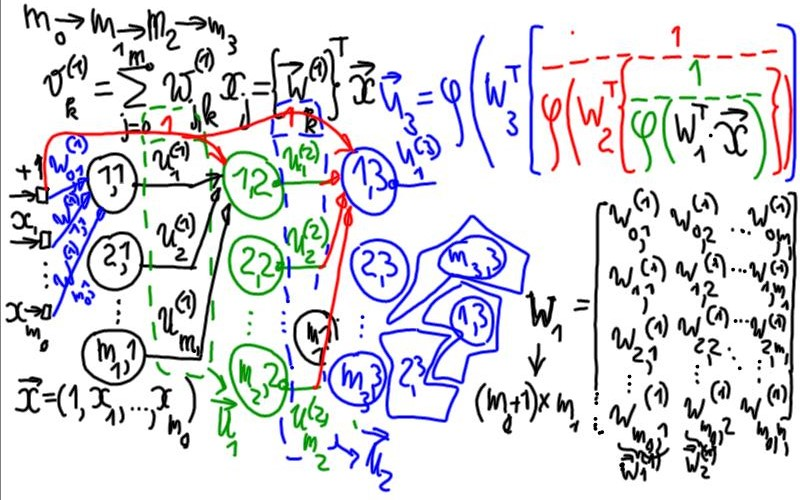
\includegraphics[width=\textwidth]{hyperflat_3_1.jpeg}
    \caption{Структура многослойного перцептрона}
    \label{hyperflat_3_1}
\end{figure}

3-слойный перцептрон содержит 0-й слой - слой источников (черные квадратики). 
Имеется $m_{0}$ входов, на которые поступают признаки 
$\vec{x} = (1, x_0, ..., x_{m_{0}})$, 3 скрытых слоя.

Примем следующие правила индексации скрытых нейронов и нейронов выходного слоя:
первый эл-т индекса - номер нейрона, второй - номер слоя: 
$m_{i,j}$  - $i$-й нейрон $j$-го скрытого слоя.

Выпишем веса нейронов $i$-го слоя в виде матрицы $W_i$, столбец которой 
$\vec{w}_i^{(k)}$ является вектором весов $i$-го нейрона $k$-го слоя.
Количество строк матрицы - количество входов слоя \glqq +1\grqq 
(на вход поступает расширенный вектор), количество столбцов - количество нейронов слоя.
Элемент матрицы $w_{i,j}^{(k)}$ - вес $i$-го входа $j$-го нейрона $k$-го слоя.
У первого скрытого слоя имеется $m_0$ входов (слой источников) 
и он содержит $m_1$ нейронов.

\begin{equation}
    W_1 = 
    \begin{pmatrix}
        w_{0,1}^{(1)} & w_{0,2}^{(1)} & \dots & w_{0,{m_1}}^{(1)} \\
        w_{1,1}^{(1)} & w_{1,2}^{(1)} & \dots & w_{1,{m_1}}^{(1)} \\
        w_{2,1}^{(1)} & w_{2,2}^{(1)} & \dots & w_{2,{m_1}}^{(1)} \\
        \vdots        & \vdots        & \ddots & \vdots           \\
        w_{{m_0},1}^{(1)} & w_{{m_0},2}^{(1)} & \dots & w_{{m_0},{m_1}}^{(1)} \\
    \end{pmatrix}
\end{equation}

Рассмотрим первый слой.
На вход каждого нейрона слоя поступает сигнал смещения $+1$, взвешиваемый 
\textit{биасом} $w_{0,i}^{(1)}$. 
Также на вход этого нейрона поступают входные признаки $x_i$, взвешиваемые 
\textit{синаптическими весами} $w_{1,j}^{(1)}$ до $w_{{m_0},j}^{(1)}$ - веса $i$-го признака $j$-го нейрона в первом слое.   
Для экономии места введём вектор синаптических весов конкретного нейрона:

\begin{equation}
    \vec{w}_j^{(k)} = 
    \begin{pmatrix}
        w_{0,j}^{(k)} & w_{1,j}^{(k)} & \dots & w_{{m_0},j}^{(k)}
    \end{pmatrix}
    ^T
\end{equation}


Индекс в скобках - номер слоя, нижний индекс - номер нейрона. Т.е., $\vec{w}_1^{(1)}$ - вектор синаптических весов 1-го нейрона 1-го слоя.

На выходе $i$-го нейрона $k$-го слоя формируется сигнал $u_i^{(k)}$. 
Выпишем формулу для вычисления сигнала на выходе 1-го нейрона 1-го слоя $u_1^{(1)}$. Опять, в скобках - номер слоя, индекс - номер нейрона.
Для этого необходимо посчитать сигнал на выходе сумматора $k$-го нейрона (\textit{индуцированного локального поля}):

\begin{myquote}
    \textit{Не очень удачно были выбраны индексы, но оставил, как на презентации}
\end{myquote}

\begin{equation}
    {v}_k^{(1)} = \sum_{j=0}^{m_0} w_{j,k}^{(1)} \cdot x_j = [\vec{w}_{k}^{(1)}]^T \cdot \vec{x}
\end{equation}


\begin{equation*}
    {v}_2^{(1)} = [\vec{w}_{2}^{(1)}]^T \cdot \vec{x}
\end{equation*}

где $j$ - номер нейрона, $k$ - номер слоя, $w_{j,k}^{(1)}$ - компоненты ..., $\vec{x}$ ---
 расширенный вектор.

Из приведённых выражений можем получить общее: $W_k^T \cdot \vec{x}$ --- совокупность элементов 
на выходе сумматоров всех нейронов $k$-го слоя.

Полученные на выходе сумматора значения подвергаются нелинейному преобразованию 
с помощью функции активации $\varphi(W_k^T \cdot \vec{x})$. Получаем совокупность 
сигналов на выходе функций активации нейронов. 
Для первого слоя: $\varphi(W_1^T \cdot \vec{x})$, для второго: $\varphi(W_2^T \cdot \vec{x})$ и т.д.

Для получения из матрицы $W_1$ матрицы $W_2$ рисуем таблицу:

\begin{center}
    Количество входов и выходов скрытых слоёв (без учёта "расширенности" векторов):

    \begin{tabular}{c | c |  c | c |}
        & 1 слой & 2 слой & 3 слой \\
        \hline
        Количество входов  & $m_0$ & $m_1$ & $m_2$ \\
        \hline
        Количество выходов & $m_1$ & $m_2$ & $m_3$ \\
        \hline
    \end{tabular}
\end{center}

Выпишем матрицу $W_2$;
\begin{equation}
    W_2 = 
    \begin{pmatrix}
        w_{0,1}^{(2)} & w_{0,2}^{(2)} & \dots & w_{0,{m_2}}^{(2)} \\
        w_{1,1}^{(2)} & w_{1,2}^{(2)} & \dots & w_{1,{m_2}}^{(2)} \\
        w_{2,1}^{(2)} & w_{2,2}^{(2)} & \dots & w_{2,{m_2}}^{(2)} \\
        \vdots        & \vdots        & \ddots & \vdots           \\
        w_{{m_1},1}^{(2)} & w_{{m_1},2}^{(2)} & \dots & w_{{m_1},{m_2}}^{(2)} \\
    \end{pmatrix}
\end{equation}

И получим выходы сумматоров нейронов второго слоя:

\begin{myquote}
    Починить расширенные вектора!
\end{myquote}

\begin{equation}
    \vec{u}_2 = W_2^T \cdot [\dfrac{1}{\varphi(W_1^T \cdot \vec{x})}]
\end{equation}


В формуле 1 в якобы числителе - добавленный первый элемент, чтобы получить расширенный вектор-столбец.

\begin{equation}
    \vec{u}_3 = \varphi(W_3^T[\dfrac{1}{\varphi(W_2^T \cdot [\dfrac{1}{\varphi(W_1^T \cdot \vec{x})}])}])
\end{equation}

Для 4-го слоя получим:

\begin{myquote}
    \textit{Выписать матрицу с рисунка для 4 слоя, поправить формулу и выписать её}
\end{myquote}

Увеличение слоёв нецелесообразно из-за рекурсивной структуры модели многослойного 
перцептрона (последовательность вложенных блоков), что приводит к уменьшению 
скорости вычисления, увеличению занимаемой памяти и накопления ошибок.
Также по мере увеличения параметров модели, возникает \textit{эффект переобучения}, 
а по мере увеличения количества слоёв количество параметров увеличивается экспоненциально.

Возможно применение альтернативных архитектур - например, сети радиальных базисных функций.
Также необходимо применение методов регуляризации, например, метод \textit{хирургии мозга} ---
исключения из каждого слоя неинформативных нейронов или целых слоёв.
Существуют методы обучения, подразумевающие цикличность.

\begin{myquote}
    \textit{Более детально см. "Нейронные сети. Полный курс" Саймона Хайкина.}
\end{myquote}

Также существует теорема, доказанная Колмогоровым, утверждающая, что многомерная 
скалярная функция может воспроизводить любую закономерность сколь угодно большой 
сложности. Теорема об универсальной аппроксимации многослойным перцептроном 
утверждает, что архитектура многослойного перцептрона \textit{теоретически} 
позволяет с любой заданной точностью синтезировать многомерную по количеству 
входов векторную функцию, что позволяет строить модели нелинейных 
дискриминантных границ в пространстве признаков и, соответственно, определять 
принадлежность данных кластерам. 




\subsection{Системный подход к синтезу алгоритмов обучения многослойного перцептрона}

Согласно системному подходу к синтезу алгоритмов обучения многослойного перцептрона, 
необходимо выполнить 3 шага:
\begin{enumerate}
    \item Выбор цели обучения;
    \item Оценка градиента средних потерь целевой функции по параметрам нейронной сети;
    \item Использование алгоритмом поиска оптимальных параметров.
\end{enumerate}

Предполагается наличие функционала качества работы системы, оптимальное значение 
которого и ищется.

\begin{figure}[htbp]
    \centering
    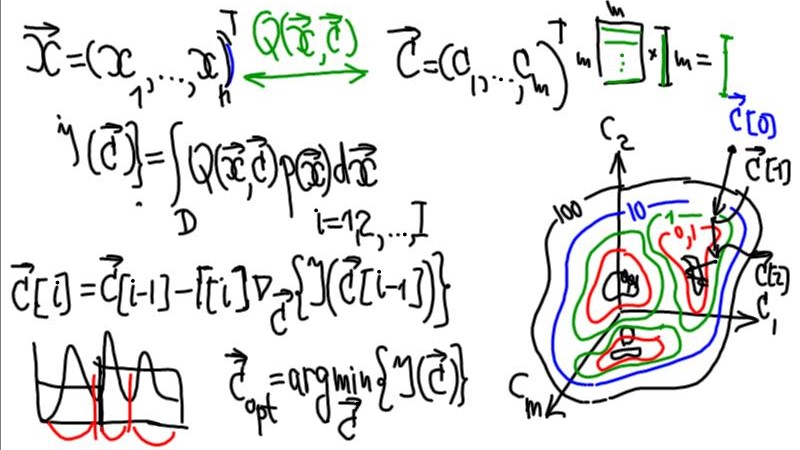
\includegraphics[height=8 cm]{hyperflat_4_1.jpeg}
    \caption{Обучение нейронной сети}
    \label{hyperflat_4_1}
\end{figure}

Будем рассматривать 3 объекта анализа
\begin{enumerate}
    \item Пространство входных воздействий $\vec{x}$ - сигналы, поступающие на вход системы 
    (обучающие и контрольные примеры), и соответствующее пространство входных воздействий, 
    в котором существует область $D$ все возможных входных воздействий;
    \item Вектор параметров системы $\vec{C}$ и пространство, ему соответствующее, 
    в которому существуют эквипотенциальные гиперповерхности, все точки которых 
    соотв. определенным значениям функционала качества. Необходимо найти 
    область минимальных/максимальных значений этого функционала качества;
    \item Функция стоимости (потерь, приобретений) $Q(\vec{x}, \vec{c})$, 
    определяющая потери/приобретения, которые можно измерить, если на вход 
    системы поступает воздействие $\vec{x}$, а система находится в в состоянии $\vec{C}$.
\end{enumerate}

Набор этих 3 объектов позволяет математически строго сформулировать выбор цели обучения 
в виде функционала средних потерь (среднего риска).
Сделать это несложно, необходимо протестировать область $D$ всех входных воздействий: 
зафиксировать $\vec{x}$ и выбрать параметры системы $\vec{C}$. 

Для каждого зафиксированного выбора параметров системы необходимо вычислить 
потери по выбранной для каждого входного воздействия и просуммировать их:

\begin{equation}
    J(\vec{C}) = \int_{D} Q(\vec{x}, \vec{C}) p(\vec{x}) d\vec{x}
    \label{eq:avg_risk}
\end{equation}

Полученное $J(\vec{C})$ - \textit{средний риск} (\textit{средние потери}), $p(\vec{x})$ --- 
весовая функция, сглаживающая аномальные значения (плотность распределения вероятностей 
входных воздействий).

На практике возможны 2 ситуации:
\begin{enumerate}
    \item Нетипичный случай полной априорной определённости - полное знание входных 
    воздействий (весовой функции $p(\vec{x})$, Типа распределения и тд.);
    \item Типичный случай - функция задана набором обучающий примеров
\end{enumerate}

Во втором случае необходимо выполнить предварительную выборочную оценку весовой функции 
$p(\vec{x})$ по набору обучающих примеров.

Однако, будем считать весовую функцию $p(\vec{x})$ известной, тогда возможно посчитать функционал 
ошибок $J(\vec{C})$.

\subsection{Алгоритм обучения нейронной сети (метод градиентного поиска)}
\begin{enumerate}
    \item Выбрать начальное приближение параметров нейронной сети $\vec{C}[0]$ 
    ($0$ - номер итерации), и оценить потери;
    \item Выбрать оптимальное направление поиска (вектор антиградиента 
    $-\nabla\vec{C}$, указывающий направление, в котором потери убывают 
    с максимальной скоростью);
    \item Выбрать шаг поиска (используется процедура стохастической 
    аппроксимации Роббенса-Монро, в соответствии с которой с каждой 
    итерацией длина шага уменьшается обратно пропорционально номеру итерации);
    \item[] В полученной точке выполняется подтверждение сходимости 
    (сравнение итераций), вычисление нового направления и шага.
    \label{en:alg}
\end{enumerate}

Процедура описывается следующим выражением:

\begin{equation}
    \vec{C}[i] = \vec{C}[i-1] - \Gamma[i] \nabla\vec{C} \{ J(\vec{C}[i-1]) \}
\end{equation}

Здесь $\Gamma[i]$ --- матрица усиления, управляющая выбором величины шага поиска.
Если она является диагональной, то по каждому признаку шаги будут независимы 
(характерно для случая гиперсфероидальной топологии гиперповерхностей равных
значений функции стоимости).

Цель обучения: 

\begin{equation}
    \vec{C}_{opt} = \arg \min_{\vec{C}} \{ J(\vec{C}) \}
\end{equation}

Существуют также методы, не требующие вычисления частной производной, ---
 метод деформируемого многогранника Нелдера-Мида (симплекс-поиск).

\begin{myquote}
    \textit{Прикладное нелинейное программирование, Химмельблау}
\end{myquote}

Обучение сводится к решению задачи оптимизации. Существуют ограничения на значения параметров 
системы в виде равенств или неравенств.

Результаты выполнения алгоритма зависят от выбора начального приближения, что приводит 
к необходимости выбора нескольких начальных приближений для обнаружения всех локальных 
минимумов. Существенное преимущество в этом случае обеспечивают генетические алгоритмы.




\section{Лекция 09.04 (дистанционная)}

\subsection{Алгоритм обучения нейронной сети для случая набора обучающих примеров}

\begin{figure}[htbp]
    \centering
    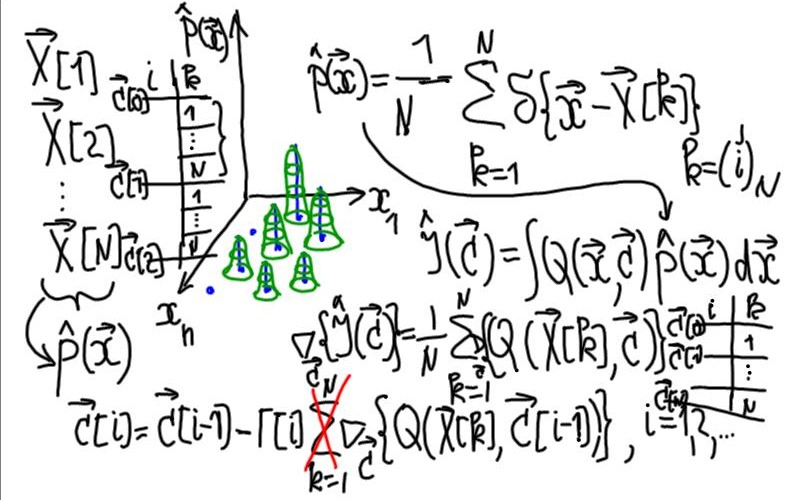
\includegraphics[height=10 cm]{hyperflat_5_1.jpeg}
    \caption{Системный подход к обучению многослойного перцептрона}
    \label{hyperflat_5_1}
\end{figure}

В подавляющем большинстве практических приложений весовая функция $p(\vec{x})$, 
входящая в выражение функционала среднего риска \ref{eq:avg_risk} задана неявным 
образом в виде набора обучающих примеров $\hat{p}(\vec{x})$.

Здесь и далее обучающие примеры, ранее обозначавшиеся $\vec{x}$, будем обозначать
$\vec{X}$. Объём выборки - $N$ обучающих примеров (см. левый столбец 
на \ref{hyperflat_5_1}), размерность пространства признаков $\{ x_1, \dots, x_n \}$ ---
$n$.

Таким образом в $x$-пространстве имеется набор обучающих примеров 
$\vec{X}[1],\dots,\vec{X}[N]$, визуализированных диаграммой рассеяния 
(график на \ref{hyperflat_5_1}). Точка задаётся радиус-вектором, набор которых
задаёт набор обучающих примеров.

Для приближения функционала среднего риска к реальности, дополним его ещё одной осью 
$\hat{p}(\vec{x})$, вдоль которой будем откладывать значения оценки весовой функции, 
где $\Hat{\textup{крышечка}}$ показывает, что это оценка.

В теории искусственного интеллекта существует огромное количество непараметрических,
параметрических и полупараметрических описаний распределений,
в т.ч. и вероятностных. Например, примером параметрического описания многомерного
распределения является модель конечной смеси стандартных распределений, для идентификации
параметров которой служат EM-алгоритмы.
Пример полупараметрической оценки --- ядерная оценка Парзена-Розенблатта,
одномерная модель ПРВ в виде гистограммы, сглаженной сдвигом (с обобщением
до многомерной модели).

\begin{myquote}
    \textit{Ссылка на книгу David Scott, Multivariate Density Estimation}
\end{myquote}




\subsubsection{Ядерная модель Парзена-Розенблатта}

Идея заключается в ассоциировании функции ядра каждой точкой в подпространстве 
признаков с каждым наблюдением (обучающим примером) --- \glqq гиперхолмы\grqq 
на рисунке \ref{hyperflat_5_1}.
Рассмотрим простейший случай, когда оценка обладает единственным параметром 
сглаживания для всех наблюдений --- \textit{неадаптивная ядерная оценка Парзена-
Розенблатта}.

Такие функции обладают важными свойствами.
Гиперобъём под поверхностью функции ядра всегда равен 1 (функция ядра интегрируема с 1).
Также, как и у любой оценки многомерного ПРВ, присутствует параметр сглаживания
(в одномерном случае --- ширина разрядного интервала,
в многомерном случае -- гиперобъём гиперпараллелепипеда), регулирующий степень 
убывания высоты холма по мере удаления текущего радиса-вектора (аргумента ПРВ)
от центра холма (выбранного обучающего примера). 

Если текущее значение совпадает с выбранным примером, то высота максимальна. 
По мере удаления от \textit{центра опорной области} (центра холма) высота асимптотически
стремится к $0$. Аналогично случаю гистограммной оценки, при стремлении параметра 
сглаживания к 0 (масштаб функции ядра нулевой) высота будет неограниченно возрастать,
а опорная область асимптотически стягиваться к 0 и приближаться к дельта-функции 
Дирака --- набору \glqq иголок\grqq единичного объёма в гиперпространстве.
Такие \glqq иголки\grqq не могут иметь общие области и, таким образом, 
ядерная оценка при таком выборе параметров превращается в \glqq лес иголок\grqq 
и (что плохо) сглаживание экспериментальных производится не будет
 --- \textit{эмпирическая оценка весовой функции}.

\begin{equation}
    \hat{p}(\vec{x}) = \dfrac{1}{N} \sum_{k=1}^{N} \delta(\vec{x} - \vec{X}[k])
    \label{eq:empirical_weight_func}
\end{equation}

Для эмпирической оценки суммируем дельта-функции, ассоциированные с обучающими примерами
и масштабируем значение в зависимости от числа обучающих примеров.

\begin{myquote}
    \textit{Обещано позже положительное свойство}
\end{myquote}

В ядерной оценке Парзена-Розенблатта увеличивается параметр сглаживания и опорная область
расширяется по мере увеличения параметра сглаживания, а высота \glqq холмов\grqq
начинает уменьшаться и ближайшие обучающие примеры начинают перекрываться, происходит
постепенное сглаживание совокупности обучающих примеров и получаем \glqq гиперрельеф\grqq.

До некоторого момента при определённом числовом диапазоне параметров 
сглаживания гиперрельеф сохраняет свою морфологию --- наблюдается определённое количество
вершин, что свидетельствует о наличии кластерной структуры в данных и характеризует
статистическую устойчивость оценки ПРВ при выборе параметра сглаживания из этого диапазона.

При дальнейшем увеличении параметра сглаживания опорные области функций-ядер начинают
чрезмерно увеличивать и кластерная структура гиперрельефа начинает
исчезать и в асимптотике стремится к плато --- равномерному распределению 
по всем признакам.

Существует набор методов, позволяющих выбрать оптимальное значение параметров сглаживания,
который позволяет обнаружить кластерную структуру, т.е. \textit{многомодовый характер} 
гиперрельефа в $n$-мерном пространстве признаков.

Один из таких методов - \textit{метод скользящей проверки} выбора оптимального параметра
сглаживания. Существуют также адаптивные ядерные оценки, в которых для каждого наблюдения
выбирается свой оптимальный параметр сглаживания и каждый \glqq гиперхолм\grqq будет
обладать своей оптимальной опорной областью (похоже на выбор характеристик масштаба 
модели конечной смеси стандартных распределений).
В ещё более сложных оценках индивидуальными являются не только параметры сглаживания,
но и модель функция ядра, например, \textit{адаптивная фильтрационная ядерная оценка
плотности распределения вероятности}. Это отдельное направление, связанное с 
построением оптимальных оценок одномерных ПРВ.

\begin{myquote}
    \textit{Есть статья на labnet.ru - Рандомизация многомерных распределений в метрике
    Махаланобиса}
\end{myquote}




\subsubsection{Интегрирование весовой функции среднего риска в конечном виде}

Конечная цель --- получить возможность проинтегрировать \ref{eq:avg_risk} в конечном 
виде, чтобы получить в конечном виде оценку среднего риска, поскольку
необходимо сформировать оценки компонентов вектора градиента и реализовать этот 
алгоритм обучения для практических приложений. 

В этом случае поможет эмпирическая оценка --- плата за попытку 
получить выражение \ref{eq:avg_risk} является грубая эмпирическая 
оценка весовой функции, которая преднамеренно игнорирует процедуру
сглаживания обучающих данных.

Преимущество --- фильтрующее свойство дельта-функции. При подстановке \ref{eq:empirical_weight_func}
в \ref{eq:avg_risk}:

\begin{equation}
    \hat{J}(\vec{C}) = \int_{D} Q(\vec{x}, \vec{C}) \hat{p}(\vec{x}) d\vec{x}
    = \dfrac{1}{N} \int_{D} Q(\vec{x}, \vec{C}) \sum_{k=1}^{N} \delta(\vec{x} - 
    \vec{X}[k]) d\vec{x}
\end{equation}

\noindent
при смене порядка суммирования и интегрирования дельта-функция \glqq профильтрует \grqq
значения весовой функции для каждого обучающего примера:

\begin{equation}
    \hat{J}(\vec{C}) = \dfrac{1}{N} \sum_{k=1}^{N} \int_{D} 
    Q(\vec{x}, \vec{C}) \cdot \delta(\vec{x} - \vec{X}[k]) d\vec{x}
\end{equation}

Произведение функции стоимости и дельта-функции, ассоциированной с конкретным обучающим
примером $Q(\vec{x}, \vec{C}) \cdot \delta(\vec{x} - \vec{X}[k])$ даст значение функции
стоимости для конкретного обучающего примера.

Таким образом, эмпирическая оценка функционала среднего риска представляет собой сумму
функции стоимости по всем обучающим примерам для выбранного вектора параметров системы,
нормированную по количеству обучающих примеров, т.е. выборочное среднее мат. ожидания
функции стоимости:

\begin{equation}
    \hat{J}(\vec{C}) = \dfrac{1}{N} \sum_{k=1}^{N} Q(\vec{X}[k], \vec{C})
\end{equation}

Применение выборочного среднего означает неробастность функции, т.е. неустойчивость
к аномалиям. Финальный алгоритм обучения будет обладать значимой шумовой компонентой 
и игнорирование влияния аномалий тоже скажется на качестве текущих оценок параметров 
обучения системы в процессе их настройки.

Поскольку вектор градиента есть набор частных производных, а операции суммирования 
и дифференцирования перестановочны, то запишем выражение для эмпирической оценки вектора
градиента:

\begin{equation}
    \nabla_{\vec{C}} {\hat{J}(\vec{C})} = \dfrac{1}{N} \sum_{k=1}^{N} \nabla_{\vec{C}}{Q(\vec{X}[k], \vec{C})}
\end{equation}




\subsubsection{Пакетный, последовательный и комбинированный режимы обучения}

Подставим полученную в конечном виде оценку градиента в синтезированный ранее алгоритм,
получим адаптированный к случаю обучения системы по набору параметров алгоритм:

\begin{equation}
    \vec{C}[i] = \vec{C}[i-1] - \Gamma[i] \sum_{k=1}^{N} \nabla\vec{C} \{ Q(\vec{X}[k], \vec{C}[i-1]) \}
\end{equation}

Пока операцию суммирования (усреднения по всем возможным значения компонент вектора 
градиента) сохраняем.

Проанализируем обучение системы при наличии этого усреднения. В этом случае процедура 
обучения реализует \textit{пакетный режим} обучения (см. \ref{table:packet_training}).

В распоряжении имеется набор из $N$ обучающих примеров, происходит инициализация алгоритма
обучения начальными значениями параметров системы. Прежде чем откорректировать начальное
приближение параметров системы в соответствии с существованием этой суммы, необходимо
перебрать все обучающие примеры, вычислить значения функции стоимости и частные 
производные для всех обучающих примеров, получить в $C$-пространстве набор направлений
оптимальных поисков (свой для каждого примера), просуммировать эти вектора, взять 
усреднённое направление поиска с отрицательным знаком, гарантирующее приемлемую скорость
убывания, выбрать величину шага и только после этого от $\vec{C}[0]$ перейти к $\vec{C}[1]$.
На следующей итерации шаги повторяются.

Пакетный режим обучения требует максимально возможной памяти.

\begin{table}[htbp]
    \centering
    \caption{Описание пакетного режима обучения}
    \label{table:packet_training}
    \begin{tabular}{c | c | c}
        Вектор параметров системы     & $i$ --- Номер итерации обучения & $k$ --- Номер обучающего примера \\\hline
        \multirow{3}{*}{$\vec{C}[0]$} & \multirow{3}{*}{1}  & 1 \\\cline{3-3}
                                      &                     & $\vdots$\\\cline{3-3}
                                      &                     & $N$ \\\hline
        \multirow{3}{*}{$\vec{C}[1]$} & \multirow{3}{*}{2}  & 1 \\\cline{3-3}
                                      &                     & $\vdots$\\\cline{3-3}
                                      &                     & $N$ \\\hline
        $\vdots$                      & $\vdots$            & $\vdots$ \\\hline
    \end{tabular}
\end{table}

Альтернативой пакетному режиму обучения является \textit{последовательный режим обучения}
(см. \ref{table:seq_training}).
Для этого опускаем операцию суммирования всех возможных направлений и после каждого
обучающего примера выполняем коррекцию:

\begin{equation}
    \vec{C}[i] = \vec{C}[i-1] - \Gamma[i] \nabla\vec{C} \{ Q(\vec{X}[k], \vec{C}[i-1]) \}
\end{equation}

при последовательном режиме обучения эффект шумовой компоненты существенно 
усиливается, поэтому на практике выбирают \glqq золотую середину\grqq, что
согласуется с процедурами сглаживания временных рядов.

\begin{table}[htbp]
    \centering
    \caption{Описание последовательного режима обучения}
    \label{table:seq_training}
    \begin{tabular}{c | c | c}
        Вектор параметров системы     & $i$ --- Номер итерации обучения & $k$ --- Номер обучающего примера \\\hline
        $\vec{C}[0]$                  & 1                   & 1 \\\hline
        $\vec{C}[1]$                  & 2                   & 2 \\\hline
        $\vdots$                      & $\vdots$            & $\vdots$\\\hline
        $\vec{C}[N]$                  & N                   & N \\\hline
    \end{tabular}
\end{table}

Выберем некоторую компоненту в параметрах системы --- временной ряд в терминологии
номера итерации обучения. Этот ВР будет иметь интересующую трендовую составляющую,
шумовою и, возможно, циклические компоненты.

Пользуясь подходами выделения трендовых компонент ВР, используем цифровую фильтрацию:
для текущего обучающего примера и нескольких предыдущих примеров (текущую и несколько
предыдущих итераций), количество которых определяет интервал сглаживания.
Обладая этой информации, можно вычислить скользящую среднюю (или экспоненциальную 
скользящую среднюю) и реализовать подавление шумовой компоненты, выделив 
трендовые составляющие.

Таким образом, \textit{комбинированный режим обучения} предполагает учёт текущего
обучающего примера и нескольких предыдущих, что обеспечивает подавление шумовой 
составляющей и циклической компоненты.




\subsection{Алгоритм обучения перцептронного нейрона}

Прежде чем переходить к алгоритму обучения многослойного перцептрона, рассмотрим
синтез алгоритмов обучения перцептронного нейрона --- основного структурного
элемента многослойного перцептрона.

\begin{figure}[htbp]
    \centering
    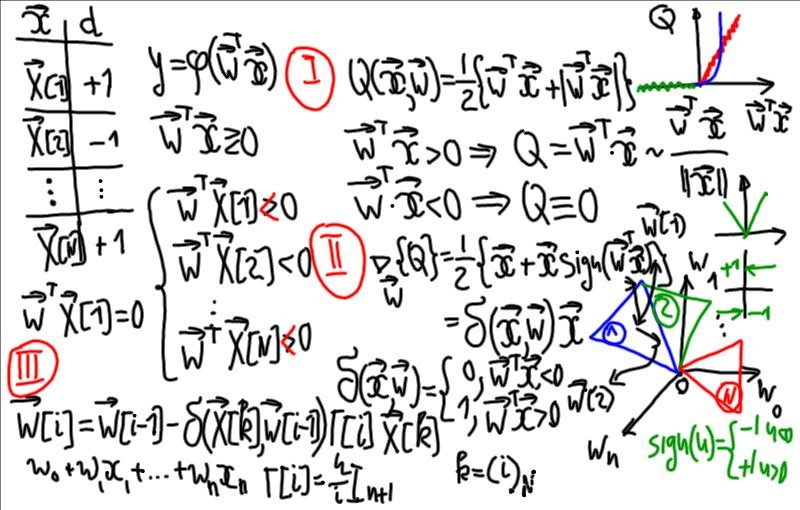
\includegraphics[height=7cm]{hyperflat_6_1.jpeg}
    \caption{Алгоритм обучения перцептронного нейрона}
    \label{hyperflat_6_1}
\end{figure}

Рассмотрим подробнее задачу \textit{дихотомии} (разделение обучающих примеров 
на 2 класса). Имеется метка $+1$ и метка $-1$ принадлежности обучающих примеров 
к 2 альтернативным классам. Рассмотрим синтез алгоритма обучения перцептронного 
нейрона в рамках задачи дихотомии. Реализуется принцип обучения с поощрением, т.е.
для настройки параметров перцептронного нейрона (биас и синаптические веса) 
применяются обучающие пары (представлены в \ref{table:learn_pairs}): обучающие примеры
$\vec{x}$ на входе перцептронного нейрона и желаемое указание (или метка класса) $d$,
поскольку перцептронный нейрон решает задачу \textit{дихотомии} .

\begin{table}[htbp]
    \centering
    \begin{tabular}{c | c}
        $\vec{x}$ --- Обучающие примеры на входе & $d$ --- желаемое указание или метка класса \\\hline
        $\vec{X}[1]$                             & $+1$ \\\hline
        $\vec{X}[2]$                             & $-1$ \\\hline
        $\vdots$                                 & $\vdots$ \\\hline
        $\vec{X}[N]$                             & $+1$ \\\hline
        
    \end{tabular}
    \caption{Обучающие пары}
    \label{table:learn_pairs}
\end{table}

Необходимо в пространстве признаков сформировать модель линейной дискриминантной
границы для того, чтобы реализовать классификацию. Как было сказано выше, существуют
2 случая: линейно разделимых и линейно неразделимых обучающих примеров.
Случай линейно разделимых обучающих примеров достаточно редко встречается
на практике, поэтому для снижения количества неизбежных ошибочных классификаций
для линейно неразделимых векторов образов была придумана \textit{система опорных векторов}.

Рассмотрим сначала простейший случай линейно разделимых векторов образов. Для этого 
понадобится математическая модель перцептронного нейрона:

\begin{equation}
    y = \varphi(\vec{w}^T \cdot \vec{x}),
\end{equation}

\noindent
причём в случае задач дихотомии функция активации $\varphi$ анализирует знак сигнала 
на выходе сумматора нейрона (линейной дискриминантной функции) и принимает вид знаковой
функции (\glqq ступенька\grqq): $\varphi(x)=-1$ для $x<0$ и $\varphi(x)=-1$ для 
$x\geqslant0$. Геометрически представляет собой гиперплоскость.

Таким образом, задачу дихотомии удобно сформулировать в терминах решения системы линейных
неравенств. С этой целью для каждой обучающей пары выпишем соответствующее неравенство:

\begin{equation}
    \begin{cases}
        \vec{w}^T \cdot \vec{X}[1] > 0 \\
        \vec{w}^T \cdot \vec{X}[2] < 0 \\
        \vdots \\
        \vec{w}^T \cdot \vec{X}[N] > 0 \\
    \end{cases}
\end{equation}

Стандартизуем систему линейных неравенств --- приведём все неравенства к знаку $<$. 
Для этого откорректируем все обучающие примеры для тех пар, которые обладают меткой
$+1$ путём домножения их на $-1$. Получим:

\begin{equation}
    \begin{cases}
        \vec{w}^T \cdot \vec{X}[1] < 0 \\
        \vec{w}^T \cdot \vec{X}[2] < 0 \\
        \vdots \\
        \vec{w}^T \cdot \vec{X}[N] < 0 \\
    \end{cases}
    \label{eq:ineq_system}
\end{equation}

Воспользуемся 3 этапами системного подхода Я.З. Цыпкина к синтезу алгоритма обучения
перцептронного нейрона:
\begin{enumerate}
    \item Сформулировать цель обучения;
    \item Найти оценки вектора градиента функции стоимости;
    \item Выписать алгоритм градиентного поиска в $C$-пространстве параметров системы
    (состоит из биаса $w_0$ и синаптических весов $w_i$).
\end{enumerate}




\subsubsection{Формулирование цели обучения}

Выберем подходящую модель функции стоимости.

\begin{myquote}
    \textit{Ссылка на книгу Ту, Гонсалес --- Принципы распознавания образов.}
\end{myquote}

В качестве цели обучения выберем среднее арифметическое линейной дискриминантной 
функции и её модуля:

\begin{equation}
    Q(\vec{x}, \vec{w}) = \dfrac{1}{2} \{ \vec{w}^T \cdot \vec{x} + \lvert \vec{w}^T \cdot \vec{x}  \rvert \}
    \label{eq:weight_func_simple}
\end{equation}

Для понимания смысла выбора модели проанализируем 2 случая:
\begin{enumerate}
    \item Неудачный выбор параметров перцептронного нейрона;
    \item Удачный выбор параметров модели.
\end{enumerate}

При неудачном выборе параметров перцептронного нейрона знак неравенства 
из \ref{eq:ineq_system} становится $>0$:

\begin{equation}
    \vec{w}^T \cdot \vec{x} >0 \Rightarrow Q = \vec{w}^T \cdot \vec{x} \sim \dfrac{\vec{w}^T \cdot \vec{x}}{\| \vec{x} \|}
\end{equation}

Т.е., для положительных значений линейной дискриминантной функции потери будут
возрастать линейно --- неудачный выбор будет \glqq наказан\grqq.

В случае удачного выбора параметров перцептронного нейрона:

\begin{equation}
    \vec{w}^T \vec{x} >0 \Rightarrow Q \equiv 0
\end{equation}

Это позволит реализовать 2 режима: \textit{принцип подкрепления} (при удачном
выборе параметров перцептронного нейрона) и \textit{принцип наказания} 
(при неудачном выборе параметров перцептронного нейрона).

В данном случае важно рассматривать выражения не в $x$-пространстве, 
а в $w$-пространстве: при попадании в область неудачных выборов в $w$-пространстве,
необходимо перейти из неё в область удачных выборов. Чем больше расстояние от текущей
точки в $w$-пространстве от отрицательной области, тем сильнее \glqq наказание\grqq.

До этого \glqq числами\grqq являлись параметры перцептронного нейрона $w_i$, а 
\glqq буквами\grqq --- обучающие признаки $x_i$. В $w$-пространстве всё наоборот,
поскольку мы обладаем набором обучающих примеров и $w_i$ --- \glqq буквы\grqq
(аргументы, решение системы линейных неравенств), а $x_i$ --- \glqq числа\grqq.





\subsubsection{Получение оценки вектора градиента}

Выпишем в явном виде скалярное произведение $\vec{w}^T \vec{x}$:

\begin{equation}
    \vec{w}^T \vec{x} = w_0 + w_1 \cdot x_1 + \dots + w_n \cdot x_n
\end{equation}

Рассмотрим частные производные этого выражения по компонентам вектора $\vec{w}$:

\begin{align*}
    \dfrac{\partial \left( \vec{w}^T \vec{x} \right)}{\partial w_0} = 1 \\
    \dfrac{\partial \left( \vec{w}^T \vec{x} \right)}{\partial w_1} = x_1 \\
    \vdots \\
    \dfrac{\partial \left( \vec{w}^T \vec{x} \right)}{\partial w_n} = x_n
\end{align*}

Получим, что градиент произведения $\vec{w}^T \vec{x}$ по параметрам перцептронного
нейрона --- это обучающий пример $\vec{x}$:

\begin{equation}
    \nabla_{\vec{w}} \{\vec{w}^T \vec{x} \} = \vec{x}
\end{equation}

При дифференцировании модуля $\lvert x \rvert$ получим:

\begin{equation}
    \dfrac{d\lvert x \rvert}{dx} =
    \begin{cases}
        1, \quad x>0 \\
        -1, \quad x<0
    \end{cases}
    \Rightarrow \dfrac{d\lvert x \rvert}{dx} = \mathrm{sign} (x)
\end{equation}

То есть:

\begin{equation}
    \dfrac{\partial \lvert \vec{w}^T \vec{x} \rvert}{\partial w_i} = x_i \cdot \mathrm{sign} (w_i \cdot x_i)
    \Rightarrow \nabla_{\vec{w}} \{\lvert \vec{w}^T \vec{x} \rvert\} = \vec{x} \cdot \mathrm{sign} \cdot (\vec{w}^T \vec{x})
\end{equation}

Получим градиент функции стоимости \ref{eq:weight_func_simple}:

\begin{equation}
    \nabla_{\vec{w}} \{Q\} = \nabla_{\vec{w}} \left[\dfrac{1}{2} \{ \vec{w}^T \cdot \vec{x} + 
    \lvert \vec{w}^T \cdot \vec{x}  \rvert \} \right] 
    = \dfrac{1}{2}  \nabla_{\vec{w}} \left[ \vec{w}^T \vec{x} \right] + 
    \nabla_{\vec{w}} \left[ \lvert \vec{w}^T \cdot \vec{x}  \rvert \right]
    = \dfrac{1}{2} \left(\vec{x} + \vec{x} \cdot \mathrm{sign} (\vec{w}^T \cdot \vec{x})\right)
\end{equation}

Введём обозначение:

\begin{equation}
    \delta (\vec{x}, \vec{w}) = \dfrac{1}{2} \left( 1 + \mathrm{sign} (\vec{w}^T \cdot \vec{x}) \right)
\end{equation}

Заметим также, что:

\begin{equation}
    \delta (\vec{x}, \vec{w}) =
    \begin{cases}
        0, \quad \vec{w}^T \cdot \vec{x} < 0 \quad \textrm{--- удачный выбор параметров перцептронного нейрона}\\
        1, \quad \vec{w}^T \cdot \vec{x} > 0 \quad \textrm{--- неудачный выбор параметров}
    \end{cases}
\end{equation}

Содержательный смысл функции $\delta (\vec{x}, \vec{w})$ --- счётчик ошибок,
накапливающий количество ошибок при неверном выборе параметров перцептронного нейрона.

Окончательно получим:

\begin{equation}
    \nabla_{\vec{w}} \{Q\} = \delta (\vec{x}, \vec{w}) \cdot \vec{x}
\end{equation}



\subsubsection{Алгоритм градиентного поиска}

Выпишем для режима последовательного обучения:

\begin{equation}
    \vec{w}[i] = \vec{w}[i-1] - \delta (\vec{X}[k], \vec{w}[i-1]) \cdot \Gamma[i] \cdot \vec{X}[k]
\end{equation}

Если $\delta (\vec{X}[k], \vec{w}[i-1]) = 0$, то параметры на предыдущей итерации были
выбраны удачно и ничего менять не надо --- \textit{фаза подкрепления}, т.е.
$\vec{w}[i] = \vec{w}[i-1]$, коррекция отсутствует.

Если для вновь поступившего обучающего примера оценка является неудачной, т.е
$\delta (\vec{X}[k], \vec{w}[i-1]) = 0$, то необходимо изменить параметры нейрона ---
\textit{фаза наказания}, осуществляется движение в направлении антиградиента так, чтобы
попасть в отрицательную зону.

В $w$-пространстве граничная гиперплоскость, соответствующая первому неравенству 
из \ref{eq:ineq_system}, делящая пространство на случай удачного и неудачного выбора,
проходит через начало координат, поскольку при $\forall w_i = 0$ 
$\vec{w}^T \cdot \vec{X}[0] = 0$. Поворот гиперплоскости (управляющие косинусы ей нормали)
определяются компонентами обучающего примера: 

\begin{equation*}
    \dfrac{\vec{X}[i]}{\|\vec{X}[i]\|}
\end{equation*}

Вся совокупность граничных гиперплоскостей для всех обучающих примеров проходят через 
начало координат, но ориентированы различным образом (см. правый нижний угол 
\ref{hyperflat_6_1}, синий --- гиперплоскость $1$-го обучающего примера, зелёный ---
--- гиперплоскость $2$-го обучающего примера, красный --- гиперплоскость $N$-го 
обучающего примера).

В случае линейно разделимых векторов образов эти плоскости (\glqq нерегулярно\grqq) 
будут расположены более-менее регулярно, а в идеальном случае --- образуют 
многогранную поверхность в виде разрезанного гиперконуса (гиперпирамиды), 
которая делит $w$-пространство на 2 зоны (положительных и отрицательных значений 
линейной дискриминантной функции).
В этом случае существует минимум одно решение системы линейных неравенств 
\ref{eq:ineq_system}.

Отталкиваясь от начального предложения, необходимо сформировать посегментную траекторию 
градиентного поиска так, чтобы, даже находясь в положительной зоне рано или поздно,
попасть в отрицательную зону $w$-пространства. 

В случае линейно неразделимых обучающих примеров \glqq фацеты\grqq будут расположены
нерегулярно (хаотически), так, что нельзя будет найти точку в $w$-пространстве, 
удовлетворяющей всем неравенствам \ref{eq:ineq_system}. Как было сказано выше,
эту задачу решает \textit{машина опорных векторов}, обеспечивающая выбор параметров
перцептронного нейрона с минимальным количеством нарушений.

В случае процедуры стохастической аппроксимации Роббенса-Монро шаг поиска выбирают,
отталкиваясь от начального приближения в направлении антиградиента пропорционально
величине $\eta$ --- \textit{параметру скорости обучения}.

\begin{equation}
    \Gamma[i] = \dfrac{\eta}{i} I_{n+1}
\end{equation}

\noindent
где $I_{n+1}$ --- единичная матрица размерности $n+1$, поскольку помимо $n$ синаптических
весов присутствует биас $w_0$.

Уменьшение шага поиска пропорциональное номеру шага обучения гарантирует сходимость метода
как минимум в случае линейно разделимых векторов образов.
Номер текущего обучающего примера $k$ выбирается, как значение целочисленной переменной $i$ 
по модулю $N$ --- остаток от деления нацело номера итерации на количество обучающих 
примеров:

\begin{equation*}
    k = (i)_N
\end{equation*}




\section{Лекция 16.04 (Опоздал на полчаса)}

% Алгоритмы обучения перцептронного нейрона в рамках задачи дихотомии
% в соответствии с системным подходом реализуют 3 этапа (см. выше )
% В пространстве параметров обучающие примеры --- это числа, гиперплоскости,
% проходящие через начало координат, пропорционально направляющим косинусам.
% Для случая линейно разделимых образов регулярная структура (разрезанная пирамида 
% в виде фацетов) делит пространство параметров на + и -. 
% В отрицательную часть необходимо стремиться.


% Сегментарная траектория поиска в области отрицательных значений. Мы
% считаем, что система неравенств имеет решение.
% Фото hyperflat_6 1-7 1. 

% Для каждого обучающего примера, фаза наказания:
% Х-числа, W-буквы. Параметр скорости - 1 - ортогонально. Параметр скорости 2 -
% зеркальное отражение. Обычно берут долю

% Была на пред. лекции
% \begin{figure}[htbp]
%     \centering
%     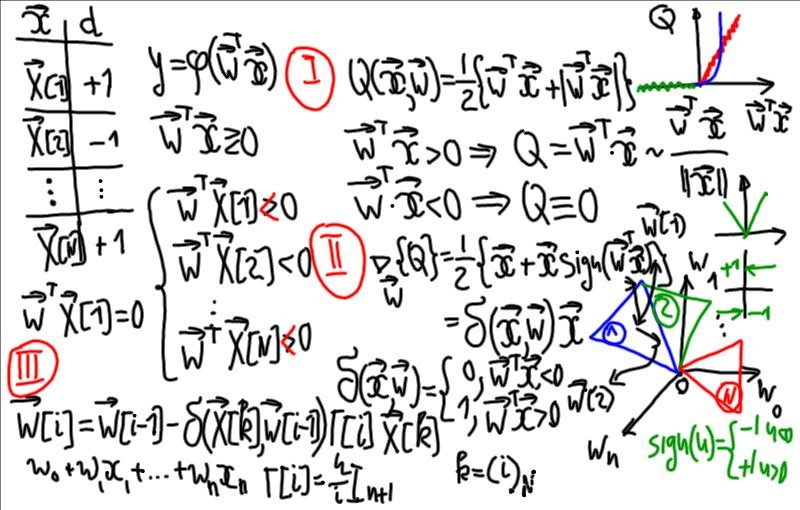
\includegraphics[height=7cm]{hyperflat_6_1.jpeg}
%     \caption{hyperflat\_6\_1}
% \end{figure}


% ------------------------------------
% В этот момент пришёл
% ------------------------------------

\begin{figure}[H]
    \centering
    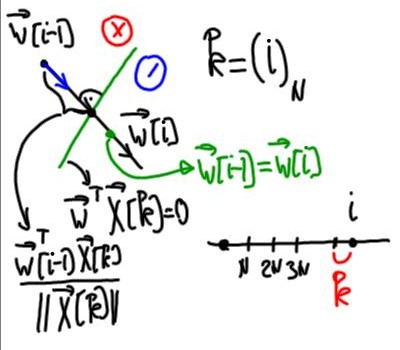
\includegraphics[height=8 cm]{hyperflat_7_1.jpeg}
    \caption{Аппроксимация многомерной скалярной функции (hyperflat\_7\_1)}
    \label{hyperflat_7_1}
\end{figure}

\textbf{Геометрическая интерпретация}
Параметр скорости обучения $\eta$ выбирают, как .. 
Переходя от одного к другому обучающему примеру, приближаемся к поверхности разрезанной 
пирамиды.

\subsection{Алгоритм обучения перцептронного нейрона с квадратичной функцией потерь}

\begin{figure}[htbp]
    \centering
    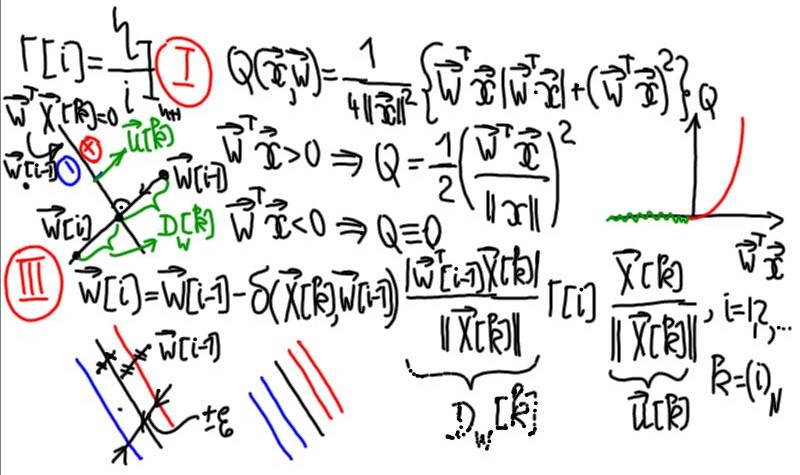
\includegraphics[height=7cm]{hyperflat_8_1.jpeg}
    \caption{Алгоритм обучения перцептронного нейрона с квадратичной функцией потерь}
    \label{hyperflat_8_1}
\end{figure}





\subsubsection{Формулирование цели обучения}

Рассмотрим новую модель функции потерь:

\begin{equation}
    Q\left( \vec{x}, \vec{w} \right) = \dfrac{1}{4 \| \vec{x} \| ^2 } 
    \left[
        \vec{w}^T \vec{x} \lvert \vec{w}^T \vec{x} \rvert +
        \left( \vec{w}^T \vec{x} \right)^2
    \right]
\end{equation}

Для неё получим:

\begin{equation}
    Q\left( \vec{x}, \vec{w} \right) =
    \begin{cases}
        \dfrac{1}{2} \left( \dfrac{\vec{w}^T \vec{x}}{\| \vec{x} \|} \right) ^2, 
        \quad \vec{w}^T \vec{x} > 0\\
        0, \quad \vec{w}^T \vec{x} < 0
    \end{cases}
\end{equation}

То есть, при неудачном выборе потери возрастают пропорционально квадрату расстояния 
текущего значения линейной дискриминантной функции от 0 --- функция потерь
квадратичная. 




\subsubsection{Вычисление оценки градиента функции ошибок}

Необходимо вычислить вектор градиента квадратичной функции ошибок:

\begin{equation}
    \nabla_{\vec{w}} \left[ Q\left( \vec{x}, \vec{w} \right) \right] =
    \nabla_{\vec{w}} 
    \left[ 
        \dfrac{1}{4 \| \vec{x} \| ^2 } 
        \left[
            \vec{w}^T \vec{x} \lvert \vec{w}^T \vec{x} \rvert +
            \left( \vec{w}^T \vec{x} \right)^2
        \right] 
    \right] =
    \dfrac{1}{4 \| \vec{x} \| ^2 } \cdot
    \left(
        \nabla_{\vec{w}}
        \left[
            \vec{w}^T \vec{x} \lvert \vec{w}^T \vec{x} \rvert
        \right] +
        \nabla_{\vec{w}}
        \left[
            \left( \vec{w}^T \vec{x} \right)^2
        \right]
    \right)
\end{equation}

\begin{myquote}
    \textit{Надо вычислить градиент функции потерь на листике}
\end{myquote}

\begin{myquote}
    \textit{Я начал выше, но идёт тяжело}
\end{myquote}




\subsubsection{Алгоритм градиентного поиска}

% Дальше пояснения ЛЛВ по поводу выражения для алгоритма
% ВЫписать выражение для алгоритма

Имея текущий обучающий пример $x_k$ и текущие параметры нейрона $\vec{W}[i-1]$,
..

\begin{myquote}
    \textit{ВЫписать выражение для градиентного поиска после слов}
\end{myquote}

В W-пространстве нормаль $\vec{u}[k]$ вычисляется как: 

\begin{equation}
    \dfrac{\vec{X}_k}{\| \vec{X}_k \|}
\end{equation}

Положим, что для $k$-го обучающего примера параметры неудачны. В этом случае опускаем перпендикуляр
к гиперплоскости и вычисляем расстояние до неё:

\begin{equation}
    D_W [k] = \dfrac{\lvert \vec{W}^T [i-1] \vec{X}[k] \rvert}{\| \vec{X}[k] \|}
\end{equation}

Долю масштаба определяют компоненты матрицы $\Gamma[i]=\dfrac{\eta}{i} I_{n\times m}$, где $I_{n \times m}$ - единичная матрица.

\begin{myquote}
    \textit{Харман, Математические основы математической вычислительной томографии, глава "РВТ"}
\end{myquote}

\begin{myquote}
    \textit{Также в книге присутствует алгоритм, в котором для гиперплоскости каждого обучающего 
    примера выбирается некая погрешность и гиперплоскость обволакивается полосой
    шириной $\pm \varepsilon$ в связи с присутствием погрешностей в "реальных" примерах.}
\end{myquote}

Для простоты анализа здесь был выбран режим последовательного обучения, однако ранее были обсуждены 
также алгоритмы
\textit{смешанного обучения}.

\begin{myquote}
    \textit{Рекомендовано выписать этот алгоритм для простой и экспоненциальной (задача со звёздочкой) 
    скользящей средней}
\end{myquote}

Здесь рассмотрен случай линейно разделимых разделимых векторов образов, исходя из предположения, что система 
линейных неравенств имеет минимум одно решение.
Иначе будет минимум одна зона в $W$-пространстве, характеризуемая количеством ошибочных классификаций 
и необходим алгоритм, строящий \textit{оптимальную гиперплоскость}.

Для \textit{оптимальной гиперплоскости} количество неизбежных ошибочных классификаций минимально. 
Такой метод был реализован Владимиров Вапником в \textit{методе опорных векторов}.

Булавский (НГУ) предложил симплекс-метод для решения несовместных систем линейных неравенств --- 
поиска компромиссного решения. 
Метод применим для случая линейно неразделимых векторов образов и является альтернативой методу 
опорных векторов. 
Метод не получил широкого распространения, имеется только препринт.


\begin{myquote}
    \textit{Препринт есть у ЛЛВ}
\end{myquote}




\subsection{Аппроксимация многомерной скалярной функции}

\begin{figure}[htbp]
    \centering
    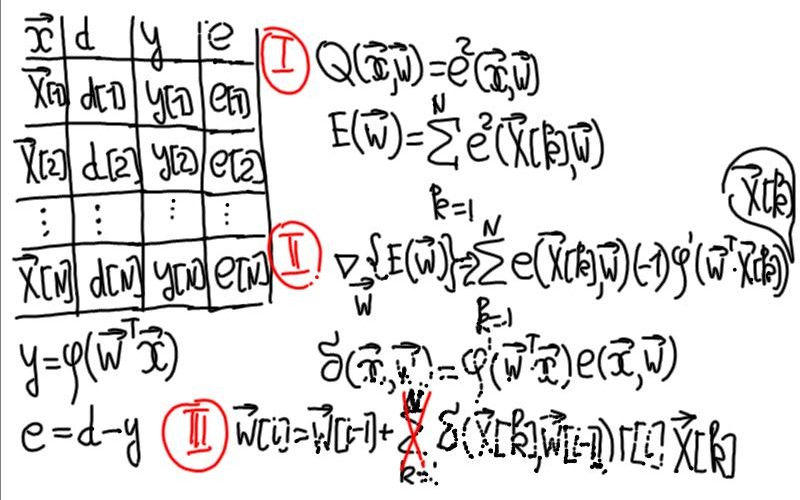
\includegraphics[height=7cm]{hyperflat_9_1.jpeg}
    \caption{Аппроксимация многомерной скалярной функции}
    \label{hyperflat_9_1}
\end{figure}

Рассмотрим альтернативную дихотомии задачу - аппроксимацию многомерной скалярной функции,  т.е.
синтез закономерности, скрытой в данных, с помощью многослойного перцептрона.
В данном случае стоит воспринимать перцептрон как устройство воспроизведения математической модели.

\begin{table}[H]
    \centering
    \begin{tabular}{| c | c | c | c |}
        \hline
        $\vec{x}$ & $d$ & $y$ & $e$ \\
        \hline
        $\vec{X}[1]$ & $d[1]$ & $y[1]$ & $e[1]$ \\
        \hline
        $\vdots$ & $\vdots$ & $\vdots$ & $\vdots$ \\
        \hline
        $\vec{X}[N]$ & $d[N]$ & $y[N]$ & $e[N]$ \\
        \hline
    \end{tabular}
    \label{table:scalar-func-table}
    \caption{Табличная форма задания многомерной скалярной функции}
\end{table}

Имеется табличная форма задания многомерной скалярной функции (\ref{table:scalar-func-table}), 
набор обучающих примеров в виде совокупности факторов (входных аргументов) $\vec{x}[i]$, $d$ ---
желаемое выходной значение скрытой закономерности, $y = \varphi (\vec{W}^T \vec{x})$ ---
фактическое значение (реакция) перцептрона и ошибка $e = d - y$.

Необходимо синтезировать математическую модель с помощью перцептронного нейрона. 
$\vec{x}$ --- обобщенный вектор образов с $+1$ в первой позиции, $\vec{W}$ ---
обобщенный вектор синаптических весов с биасом в первой позиции.

Будем выполнять задачу согласно этапам системного подхода.



\subsubsection{Выбор модели фунции стоимости}

Выберем квадратичную функцию ошибок:

\begin{equation}
    Q(\vec{x}, \vec{W}) = e^2(\vec{x}, \vec{W})
\end{equation}

Тогда средние потери будут равны:
    
\begin{equation}
    E(\vec{W}) = \sum_{k=1}^{T} e^2 (\vec{X}[k], \vec{W})
    \label{eq:sum-err}
\end{equation}



\subsubsection{Поиск градиента функции ошибок}

Необходимо найти в $W$-пространстве такую точку, которая минимизировала бы суммарную 
энергию ошибок $E(\vec{W})$ \ref{eq:sum-err}.
\begin{equation}
    \nabla_{\vec{w}} \{ E(\vec{W}) \} = 2 \sum_{k=1}^{N} e (\vec{X}[k], \vec{W}) \cdot (-1)
    \cdot \varphi ' (\vec{W}^T \cdot \vec{X}[k]) \vec{X}[k]
\end{equation}

В первую очередь интересно произведение первой производной функции активации и функции ошибки, 
которую обозначим $\delta(\vec{x}, \vec{W})$:
\begin{equation}
    \delta(\vec{x}, \vec{W}) = \varphi ' (\vec{W}^{T} \cdot \vec{x}) \cdot e(\vec{x}, \vec{W})
    \label{eq:local_grad}
\end{equation}
\noindent
и будем называть \textit{локальным градиентом}. 
Он введён, поскольку при выполнении поиска выгоднее находиться в области ненулевых значений
функции активации (иначе итерация "пропадает").



\subsubsection{Применение алгоритма градиентного поиска}

Распишем алгоритм градиентного поиска (пакетный режим):
\begin{equation}
    \vec{W}[i] = \vec{W}[i-1] + \sum_{k=1}^{N} \delta(\vec{X}[k], \vec{W}[i-1])\cdot \vec{\Gamma[i]} \cdot \vec{X}[k]
\end{equation}

\begin{myquote}
    Рекомендовано выписывать алгоритм слева направо - скаляр, матрица, вектор.
\end{myquote}

Для усиления шумового эффекта игнорируется усреднение по всем примерам (удаление знака суммы) и выполняется 
пересчёт после каждого нового значения - последовательное обучение:
\begin{equation}
    \vec{W}[i] = \vec{W}[i-1] + \delta(\vec{X}[k], \vec{W}[i-1])\cdot \vec{\Gamma[i]} \cdot \vec{X}[k]
    \label{eq:delta-rule}
\end{equation}
Здесь $\delta(\vec{X}[k], \vec{W}[i-1])$ -- локальный градиент \ref{eq:local_grad}. Режим последовательного обучения 
реализует \textit{оптимизирующий алгоритм Уидроу-Хоффа} \ref{eq:delta-rule}, 
иначе называемый \textit{дельта-правилом}.

При введении сглаживания с помощью модели EMA получим \textit{обобщённое дельта-правило}.



\subsection{Алгоритм обратного распространения ошибок обучения многослойного перцептрона}

\begin{myquote}
    \textit{Lec\_neuro\_08.docx}
\end{myquote}

Основным параметром алгоритма обучения Уидроу-Хоффа является ошибка реакции, которая 
недоступна при обучении нейронов скрытых слоёв.
Эту проблему решает алгоритм обратного распространения ошибок.

Упростим схему индексации нейронов (см. \ref{hyperflat_10_1}):

\begin{figure}[htbp]
    \centering
    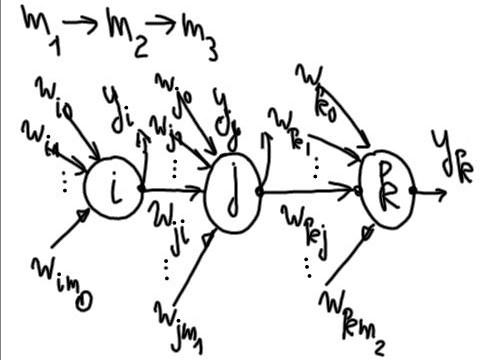
\includegraphics[width=7cm]{hyperflat_10_1.jpeg}
    \caption{Новая схема индексации нейронов}
    \label{hyperflat_10_1}
\end{figure}

Для этого примем следующие соглашения:
\begin{enumerate}
    \item Для обозначения 1-го скрытого слоя используем символ $i$, нейроны 2-го скрытого слоя 
    обозначим символами $j$, выходные нейроны обозначим символами $k$, $l$ - символ линейных 
    нейронов 0-го слоя.
    \item Связь между нейронами младшего и старшего слоя (синаптический вес) --- $W{ji}$, 
    $j$ --- символ нейрона старшего слоя, $i$ --- символ нейрона младшего слоя, 
    для биаса второй индекс $0$.
    \item Во входном слое $m_0$ нейронов (функциональных входов), во 2-м слое 
    $m_1$ нейронов, в 3-м слое $m_2$ нейронов.
\end{enumerate}

Алгоритм обратного распространения содержит 2 вычислительных этапа
\begin{enumerate}
    \item \textbf{Этап прямого распространения.} В соответствии с математической моделью многослойного 
    перцептрона можем распространить все сигналы в прямом направлении --- посчитать фактические 
    реакции нейронов скрытых слоёв и выходные реакции нейронов. 
    
    В финале этого этапа обладаем выходными реакциями нейронов, на основе которых можно 
    вычислить сигналы ошибок и локальные градиенты, а значит, применить дельта-правило 
    и скорректировать параметры нейронов выходного слоя.
    \item \textbf{Этап обратного распространения.} 
    На этом этапе распространяются сигналы ошибок для нейронов скрытых слоёв.
\end{enumerate}



\subsubsection{Этап прямого распространения}

Этап начинается с расчёта фактических реакций на выходе нейронов 1-го скрытого слоя. 

Рассчитаем сигнал на выходе сумматора текущего $i$-го нейрона на выходе 1-го скрытого слоя, 
на вход которого  поступает сигнал смещения \glqq +1\grqq, взвешиваемый биасом, и входные признаки 
$x_m0$, взвешиваемые синаптическим весом $w_{im_0}$.

На выходе сумматоров получим:

\begin{equation}
    v_i (n) = \sum_{L=0}^{m_{0}} w_{il}(n) x(n)
\end{equation}

\noindent
$n$ - номер итерации.

Подвергаем его нелинейному преобразованию и получаем реакции на выходе нейронов 1-го скрытого слоя:

\begin{equation}
    y_i(n) = \varphi (v_i(n)), \quad i=\overline{1,m_1}
\end{equation}

Посчитаем сигналы на выходе сумматоров нейронов 2-го скрытого слоя:

\begin{equation}
    v_j (n) = \sum_{i=0}^{m_{1}} w_{ji}(n) y_i(n)
\end{equation}

На выходе нейронов 2-го скрытого слоя после нелинейного преобразования:

\begin{equation}
    y_j(n) = \varphi (v_j(n)), \quad j=\overline{1,m_2}
\end{equation}

Аналогично на выходе сумматоров нейронов 3-го скрытого слоя:

\begin{equation}
    v_k (n) = \sum_{j=0}^{m_{2}} w_{kj}(n) y_j(n)
\end{equation}

На выходе нейронов 3-го скрытого слоя после нелинейного преобразования:

\begin{equation}
    y_k(n) = \varphi (v_k(n)), \quad k=\overline{1,m_3}
\end{equation}

Зная фактические реакции выходных нейронов, вычислим набор ошибок:

\begin{equation}
    e_{k}(n) = d_k(n) - y_k(n)
\end{equation}

Вычисляем величину локального градиента выходных нейронов:

\begin{equation}
    \delta_k(n) = \varphi^{\prime}(v_k(n))\cdot e_k(n)
\end{equation}

Алгоритм коррекции $k$-го выходного нейрона:

\begin{equation}
    w_{kj}(n) = w_{kj}(n-1) + \dfrac{\eta}{N} \cdot \delta_{k}(n) \cdot y_j(n), k=\overline{1,m_3}
\end{equation}

Этап прямого распространения закончен.




\subsubsection{Этап обратного распространения}

В соответствии с методом потоковых графов, разработанным Станиславом Осовским и описанным в книге
\glqq Нейронные сети для обработки информации\grqq, любую сеть можно представить в виде набора графов,
 имеющих узлы (сигналы) и рёбра (направления распространения сигналов и коэффициенты усиления).
Если рёбра сходятся в одном узле, то это означает суммирование соответствующих сигналов.

\begin{figure}[H]
    \centering
    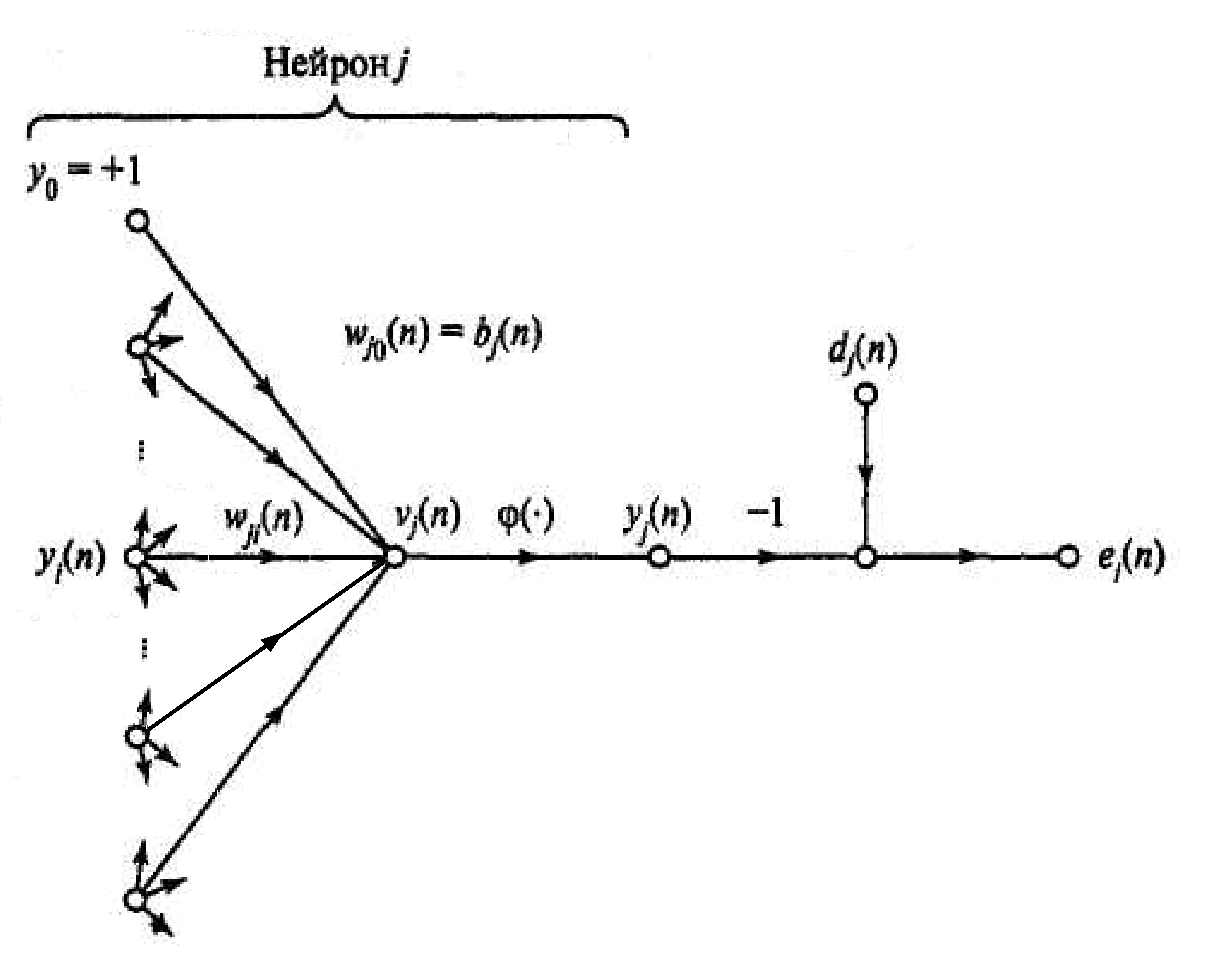
\includegraphics[height=5cm]{lec_neuro_08_4_3.png}
    \caption{Граф передачи сигнала в пределах $j$-го нейрона}
    \label{lec_neuro_08_4_3}
\end{figure}

Для нейронов выходного слоя имеем сигналы ошибки $e_1(n),\dots,e_k(n),\dots,e_{m_3}$, которые 
умножаются на вычисленные значения функции активации $\varphi^{\prime}(v_k(n))$ и получаем значения 
локальных градиентов выходных нейронов $\delta_k(n)$, а затем используем алгоритм обратного 
распространения ошибок.

\begin{figure}[htbp]
    \centering
    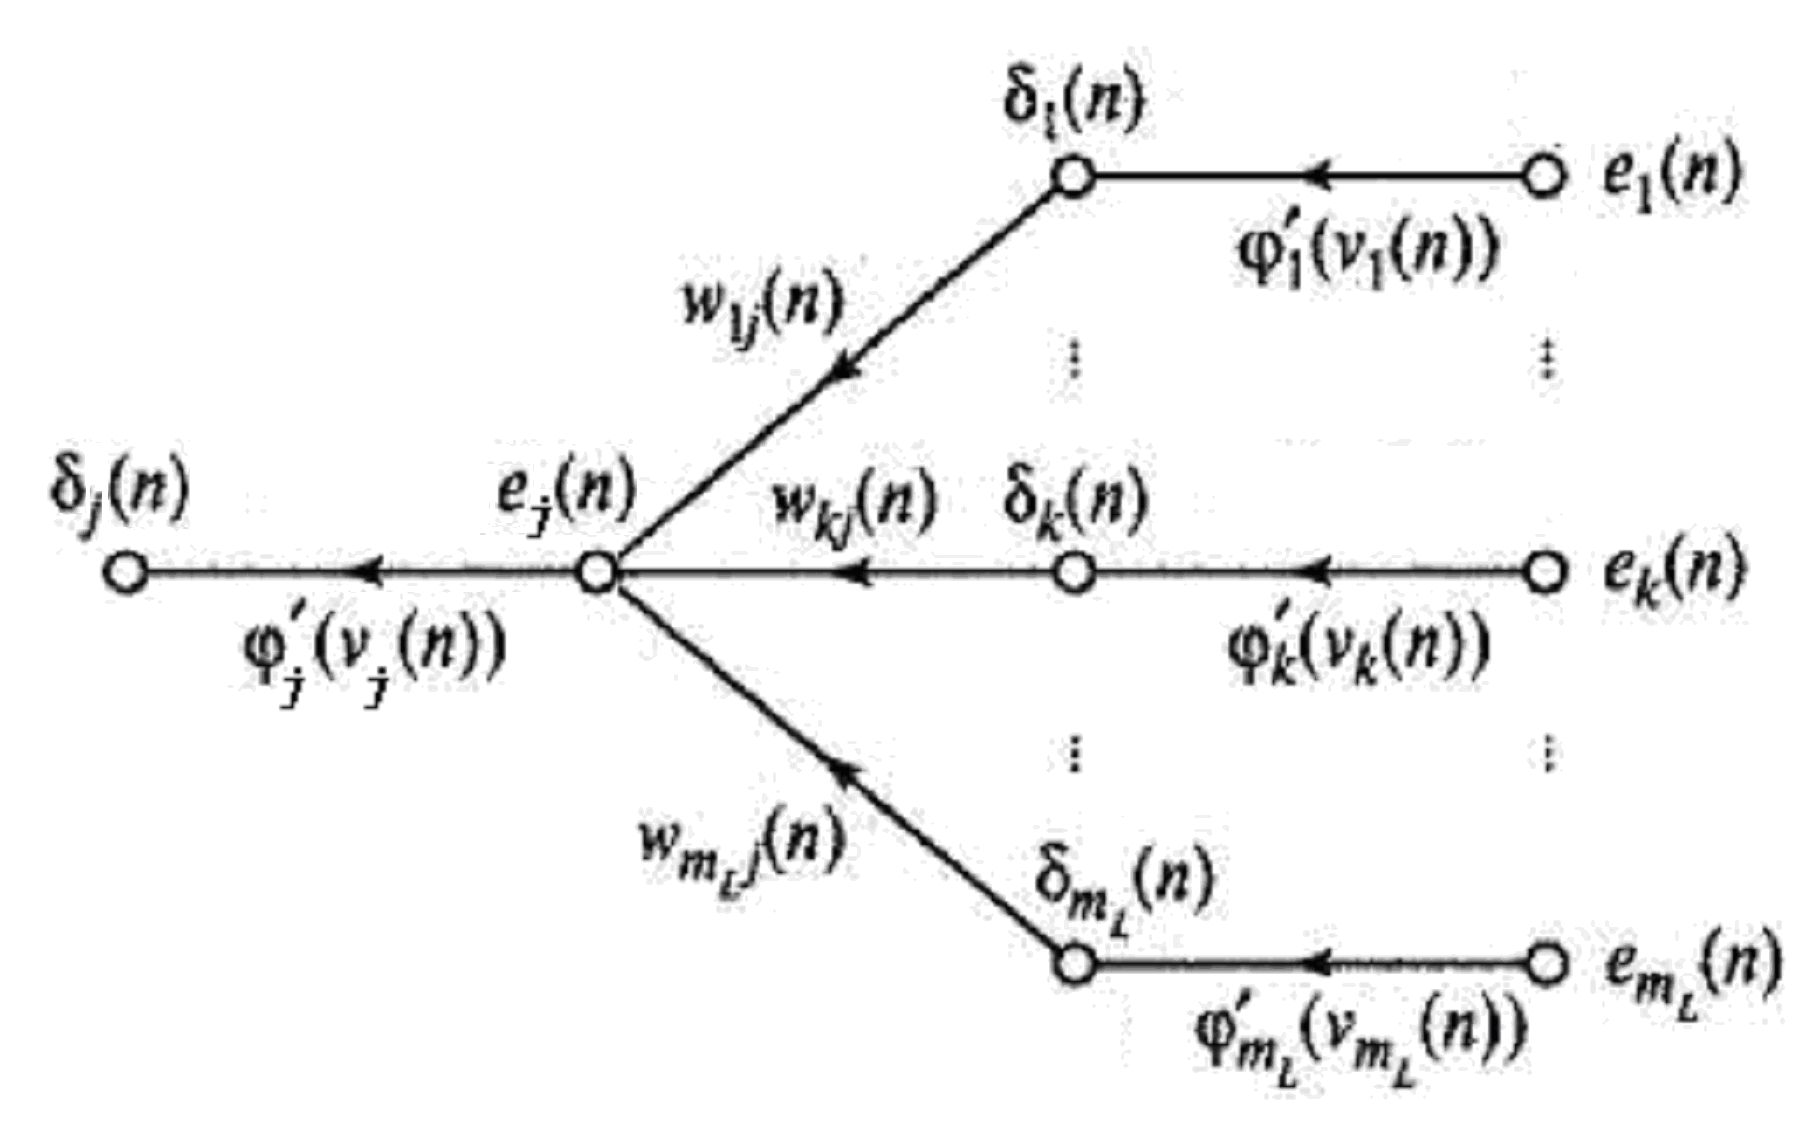
\includegraphics[height=5cm]{lec_neuro_08_4_5.png}
    \caption{Направление двух потоков сигналов в многослойном перцептроне}
    \label{lec_neuro_08_4_5}
\end{figure}

Основной результат заключается в правиле вычисления ошибок для нейронов младшего слоя. 
Показано, что сигнал ошибки может быть вычислен в виде взвешенной суммы локальных градиентов
нейронов n-го слоя:

\begin{equation}
    e_j(n) = \sum_{k=1}^{m_3} w_{kj}(n) \delta_k (n)
\end{equation}

\begin{myquote}
    \textit{Возможно, суммирование должно быть от 0.}
\end{myquote}

Вычислив ошибку для нейронов второго слоя, вычислим для него локальный градиент, т.е. 
распространим ошибку на шаг назад:

\begin{equation}
    \delta_j(n) = e_j(n) \cdot \varphi^{\prime} (v_j(n))
\end{equation}

Значит, возможно произвести \glqq редактирование\grqq синаптических весов нейронов второго слоя. Т.е.:

\begin{equation}
    w_{ji}(n) = w_{ji}(n-1) + \dfrac{\eta}{N} \cdot \delta_j \cdot y_i(n)
\end{equation}

Для нейронов первого скрытого слоя:

\begin{equation}
    e_i(n) = \sum_{j=1}^{m_2} w_{ji}(n) \delta_j
\end{equation}

\begin{myquote}
    \textit{Возможно, суммирование должно быть от 0.}
\end{myquote}

\begin{equation}
    \delta_i(n) = e_i(n) \cdot \varphi^{\prime} (v_i(n))
\end{equation}

Для входного слоя получим:

\begin{equation}
    w_{il}(n) = w_{il}(n-1) + \dfrac{\eta}{N} \cdot \delta_i \cdot x_l
\end{equation}

Произошло распространение ошибок и локального градиента в обратном направлении, что
позволило применить обычное дельта-правило.



\section{Лекция 23.04 (пропустил)}
\subsection{Практические рекомендации по улучшению сходимости алгоритма обратного распространения ошибок}


\subsection{Выбор начального приближения для биаса и синаптических весов}




\section{Лекция 07.05}

\subsection{Сеть главных компонент}

\subsubsection{Метод главных компонент (МГК)}

\begin{myquote}
    \textit{Lec\_Neuro\_04.docx}
\end{myquote}

\begin{figure}[htbp]
    \centering
    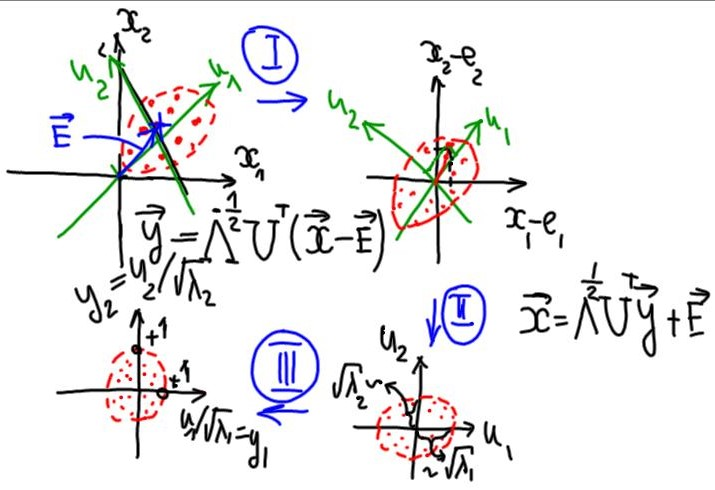
\includegraphics[height=6cm]{hyperflat_11_1.jpeg}
    \caption{Метод главных компонент}
    \label{hyperflat_11_1}
\end{figure}

При решении задач распознавания образов на первом этапе формируется пространство 
исходных признаков, которое обычно обладает  следующими недостатками:

\begin{enumerate}
    \item Избыточность исходного списка признаков, поскольку он формулируется экспертным 
    (эмпирическим) методом.
    \item Значимая корреляция исходных признаков (содержание неравных долей информации
    об объекте анализа)
\end{enumerate}

Одним из инструментов анализа морфологии такого пространства является анализ диаграммы рассеяния,
которая может демонстрировать явные направления, вдоль которых степень свободы (рассеяния)
значима, т.е., точки в пространстве образуют эллипсоид. Э является признаком значимой корреляции.

Для анализа пространства применяется ковариационная матрица исходных признаков, в которой 
прежде всего интересны собственные вектора и собственные значения.

Существует 2 группы собственных значений: 

\begin{enumerate}
    \item \textbf{Значимые} ($\gg0$). Образуют \textit{сигнальное подпространство},
        размерность (количество степеней свободы) которого определяется рангом $M$ 
        ковариационной матрицы обучающих примеров.
        Также определяют энергию сигнального подпространства, поскольку собственные значения 
        являются аналогом дисперсии, и количество степеней свободы.
    \item \textbf{Малозначимые} ($\approx 0$). Образуют \textit{шумовое подпространство},
        порождённое ошибками измерений и вычислений.
\end{enumerate}

Согласно МГК собственные вектора матрицы ковариации исходных признаков определяют новый
базис (как было показано Пирсоном), а ошибка описания исходных признаков с помощью МГК
определяется суммой малозначимых собственных значений.

\begin{figure}[htbp]
    \centering
    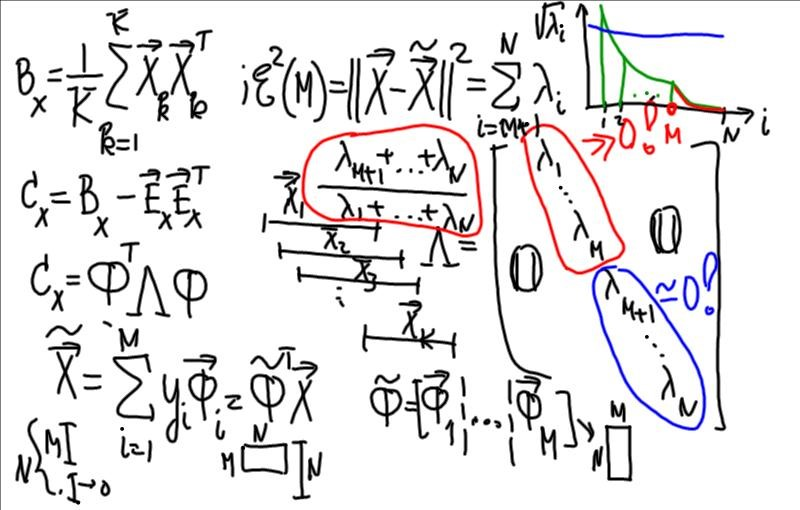
\includegraphics[height=6cm]{hyperflat_12__1.jpeg}
    \caption{Метод главных компонент (продолжение)}
    \label{hyperflat_12__1}
\end{figure}

Относительная ошибка определяется как:
\begin{equation}
    \dfrac{\lambda_{M+1}+\dots+\lambda_{M+1}}{\lambda_1+\dots+\lambda_M}
\end{equation}

То есть, задавшись допустимым значением ошибок описания, можно получить критерий отбора
собственных значений.




\subsubsection{Сеть главных компонент (введение)}

Сеть главных компонент в процессе обучения по набору непомеченных обучающих примеров
должна выдать направляющие косинусы осей сигнального подпространства (компоненты собственных
векторов), а совокупность фактических реакций нейронов сети главных компонент дать оценки 
дисперсий (оценки собственных значений), что позволит ортогонально спроецировать исходные
данные на оси сигнального подпространства. 
Задача упрощается в случае, если корреляция значима, поскольку тогда эффективный ранг 
будет на порядок меньше ранга пространства исходных признаков.

Аналогично МГК функционирует и в задачах прогнозирования.

В основе сети главных компонент лежат выборочные оценки направляющих косинусов собственных
векторов сигнального подпространства и оценки собственных значений, определяющихся
ковариационной матрицей (второй центральный момент). В литературе ковариация и корреляция
в русской и иностранной литературе альтернативны (ковариация --- correlation).
Основой выборочного оценивания является корреляционное произведение.




\subsubsection{Гипотеза Хебба (принцип самоусиления (корреляции))}

Правило коррекции синаптических весов, устанавливающее связь между входным сигналом
и его реакцией в виде корреляционного произведения в простейшей форме:
\begin{equation}
    \Delta w_{kj} (n) = \eta \cdot y_k(n) \cdot x_j(n)
\end{equation}

\noindent
иначе называемое \textit{правилом обучения синапса Хебба}. 
Здесь $x_j$ --- сигнал на входе линейного нейрона от $j$-го исходного признака, $y_k$ --- 
сигнал на выходе $k$-го нейрона, $\eta \in \left[0, 1\right]$ --- параметр скорости
обучения.

\begin{figure}[htbp]
    \centering
    \includegraphics[height=5cm]{lec_neuro_04_2_3.png}
    \caption{Иллюстрация принципов Хебба и ковариации}
    \label{lec_neuro_04_2_3}
\end{figure}

Зависимость корректирующего значения $\Delta w_{kj} (n)$ от выходного сигнала $y_k$
представлена на \ref{lec_neuro_04_2_3}. Угловой коэффициент для гипотезы Хебба равен
$\eta \cdot x_j$.
Видим, что правило Хебба не вводит ограничение на значение синаптических весов, которые могут 
возрастать бесконечно, что приводит к состоянию \textit{насыщения сети} 
(состояние, при которой выходные значения ИНС нечувствительны к изменению исходных признаков).




\subsubsection{Принцип ковариации}

Для стабилизации весов необходимо ввести обратную связь и вместо \textit{принципа 
самоусиления (корреляции)} ввести принцип конкурентности --- \textit{принцип ковариации}.

Для этого правило Хебба модифицируют центрированием обучающих примеров --- происходит параллельный 
перенос системы координат исходных признаков в центр группировки обучающих примеров 
(см. прошлое занятие). Тогда получаем:
\begin{equation}
    \Delta w_{kj} = \eta \left( x_j - \bar{x} \right) \left( y_k - \bar{y} \right)
\end{equation}

\noindent
где $\bar{x}$ и $\bar{y}$ --- усредненные по времени значения предсинаптического $x_j$ 
и постсинаптического $y_k$ сигналов.

Теперь возможны и отрицательные корректирующие значения и существует \textit{точка баланса},
что видно для соответствующей прямой на \ref{lec_neuro_04_2_3}. 




\subsection{Метод настройки весов для сети главных компонент}

Линейный нейрон, являющийся структурных элементом сети главных компонент, называют 
\textit{фильтром Хебба}.
Несмотря на простоту, в синаптических весах фильтра Хебба сохраняются 
направляющие косинусы осей в пространстве главных компонент.

\begin{myquote}
    \textit{Lec\_Neuro\_14.docx}
\end{myquote}



\subsubsection{Правила обучения линейного нейрона}

Как было отмечено выше, синаптические веса линейного нейрона по сути своей являются 
направляющими косинусами оси в пространстве исходных признаков.

\begin{figure}[htbp]
    \centering
    \includegraphics[height=4cm]{lec_neuro_14_8_5.png}
    \caption{Граф линейного нейрона}
    \label{lec_neuro_14_8_5}
\end{figure}

Рассмотрим модель линейного нейрона (представлена на \ref{lec_neuro_14_8_5}):
\begin{equation}
    y = \sum_{i=1}^m w_i x_i
\end{equation}

\noindent
где $w_i$ --- синаптические веса (всего $m$ штук), $n$ --- итерация обучения.

\begin{myquote}
    \textbf{Важно!
    Здесь отсутствует сигнал стандартного смещения $+1$ в отличие от перцептронного нейрона.}
\end{myquote}

В рамках гипотезы корреляции (согласно правилу Хебба):
\begin{equation}
    w_i (n) = w_i (n-1) + \eta \cdot y(n-1) \cdot x_i(n-1), \quad i=1, 2, \dots, m
\end{equation}
\noindent
где $n$ --- дискретное время, $\eta$ --- параметр скорости обучения.

Здесь реализован только \textit{принцип самоусиления}, что нас не устраивает. 
Необходимо ввести \textit{эффект конкуренции} между синаптическими весами: между собой они могут 
соревноваться, но при этом длина вектора синаптических весов всегда должна быть 
равна $1$, т.е. геометрически синаптические веса приобретают смысл направляющих косинусов.

Для этого после каждой итерации будем проводить нормировку, если совокупность весов не 
образует вектор единичной длины:
\begin{equation}
    w_i(n) = \dfrac{w_i(n-1) + \eta \cdot y(n-1) \cdot x_i(n-1)}
                   {\sqrt{\sum_{i=1}^{m} \left[ w_i(n-1) + \eta \cdot y(n-1) \cdot x_i(n-1) 
                                         \right] ^2}}
\end{equation}

В результате нормировки правило обучения становится нелинейным.
Поэтому применим методы линеаризации: аппроксимируем нелинейную зависимость рядом (Маклорена 
или Тейлора), степень аргумента которого будет убывать достаточно быстро.
В качестве аргумента используем применим параметр скорости обучения $\eta \in [0,1]$.

Необходимо вычислить набор частных производных по $\eta$ и их значения при $\eta=0$,
чтобы получить полином, у которого отбросим степени, старше первой (для ряда Маклорена). 
Итого получим:
\begin{equation}
    w_i(n) = w_i(n-1) + \eta \cdot y(n-1) \left[ x_i(n-1) - y(n) \cdot w_i(n-1) \right]
\end{equation}

Это полученное линеаризованное правило обучения синаптических весов линейных нейронов,
реализующее оба принципа (самоусиления и конкуренции), иногда называют \textit{правилом Ойа}.

Данное правило обучения в итоге выдаёт наибольшее собственное значение ковариационной матрицы
обучающих примеров, а веса являются направляющими косинусами.
Для понимания этого реализуем матричную формулировку алгоритма.




\subsubsection{Матричная формулировка алгоритма Ойа}

Для входного вектора исходных признаков $\vec{x}(n)$ и вектора синаптических весов $\vec{w}(n)$
введём следующие обозначения:
\begin{align}
    \vec{x}(n) &= \left[ x_1(n), x_2(n), \dots, x_m(n) \right]^T \\
    \vec{w}(n) &= \left[ w_1(n), w_2(n), \dots, w_m(n) \right]^T
\end{align}

Тогда выходная реакция линейного нейрона и правило его обучения:
\begin{align}
    y(n) &= \vec{x}^T(n) \cdot \vec{w}(n) = \vec{w}^T(n) \cdot \vec{x}(n) \label{eq:neuron_react_vec}\\
    \vec{w}(n) &= \vec{w}(n-1) + \eta \cdot y(n-1) \left[ \vec{x}(n-1) - y(n) \cdot \vec{w}(n-1) \right]
    \label{eq:oya_rule_vec}
\end{align}

Подставим в правило Ойя \ref{eq:oya_rule_vec} фактическую реакцию нейрона (различные представления
для двух вхождений в формулу \ref{eq:neuron_react_vec}) и получим:
\begin{equation}
    \vec{w}(n) = \vec{w}(n-1) + \eta \cdot y(n-1)
        \left[ 
            \vec{x}(n-1) \cdot \vec{x}^T(n-1) \cdot \vec{w}(n-1) -
            \vec{w}^T(n-1) \cdot \vec{x}(n-1) \cdot \vec{x}^T \cdot \vec{w}(n-1) \cdot \vec{w}(n-1) 
        \right]
\end{equation}

Здесь $\vec{x}(n) \cdot \vec{x}^T(n)$ --- \textit{элементарная корреляционная матрица},
квадратная матрица размерности $m \times m$.

Введём замены:
\begin{align}
    \vec{h}(\vec{w}(n), \vec{x}(n)) &= 
    \left[ 
        \vec{x}(n) \cdot \vec{x}^T(n) \cdot \vec{w}(n) -
        \vec{w}^T(n) \cdot \vec{x}(n) \cdot \vec{x}^T \cdot \vec{w}(n) \cdot \vec{w}(n) 
    \right] \\
    \vec{\eta} (n) &= \eta \cdot y(n)
\end{align}

Получим:
\begin{equation}
    \vec{w}(n) = \vec{w}(n-1) + \vec{\eta} (n-1) \cdot \vec{h}(\vec{w}(n-1), \vec{x}(n-1)),
    \quad n = 0,1,2,\dots
\end{equation}

Это нелинейное стохастическое разностное уравнение. 

По мере обучения объёма обучающих 
примеров переходим к непрерывному времени и разностное уравнение превращается в систему 
линейных ДУ:
\begin{equation}
    \dfrac{d}{dt} \vec{w}(t) = \langle \vec{h} (\vec{w}(t)) \rangle
\end{equation}

При этом используем обычную выборочную среднюю по матрице набора обучающих
примеров $\vec{X}$ (по всем реализациям $\vec{x}$):
\begin{equation}
    \langle \vec{h}(\vec{w}) \rangle = \lim_{n \to \infty} E\left[ h(\vec{w}, \vec{X}) \right]
\end{equation}

Усредняя функцию коррекции $\vec{h}(\vec{w}, \vec{x})$ по столбцам матрицы обучающих примеров:
\begin{equation}
    \vec{h}(\vec{w}, \vec{x}) = \vec{x}(n) \cdot y(n) - y^2(n) \cdot \vec{w}(n) =
    \vec{x}(n) \cdot \vec{x}^T(n) \cdot \vec{w}(n) - 
    \left[ \vec{w}^T(n) \cdot \vec{x}(n) \cdot \vec{x}^T(n) \cdot \vec{w}(n) \right] \vec{w}(n)
    \label{eq:avg_corr_func}
\end{equation}

В квадратных скобках \ref{eq:avg_corr_func} --- квадратичная форма (по определению положительна).

Усредняя \ref{eq:avg_corr_func} по множеству набора обучающих примеров, получим:

Усредняя функцию коррекции $\vec{h}(\vec{w}, \vec{x})$ по столбцам матрицы обучающих примеров:
\begin{equation}
    \langle \vec{h} \rangle = \lim_{n \to \infty} E
    \left[
        \vec{X}(n) \cdot \vec{X}^T(n) \cdot \vec{w}(n) - 
        \left( 
            \vec{w}^T(n) \cdot \vec{X}(n) \cdot \vec{X}^T(n) \cdot \vec{w}(n) 
        \right)
        \vec{w}(n)
    \right] =
    \mathbf{R}\cdot \vec{w}(\infty) -
    \left[
        \vec{w}^T(\infty) \cdot \mathbf{R} \cdot \vec{w}(\infty)
    \right] \vec{w}(\infty)
\end{equation}

\noindent
где $\mathbf{R}$ --- матрица корреляции исходных данных, $\vec{w}(\infty)$ --- предельное 
значение вектора синаптических весов

Итого получим систему ЛДУ: 
\begin{equation}
    \dfrac{d}{dt} \vec{w}(t) =  \langle \vec{h} (\vec{w}(t)) \rangle = 
    \mathbf{R}\cdot \vec{w}(t) - \left[ \vec{w}^T(t) \cdot \mathbf{R} \cdot \vec{w}(t) \right] \vec{w}(\infty)
\end{equation}

\noindent
решение которой известно:
\begin{equation}
    \lim_{n \to \infty} \vec{w}(n) = \vec{q}_1
\end{equation}

\noindent
где $\vec{q}_1$ --- оценка первого собственного вектора. Считаем свойство фильтра Хебба доказанным.

Для существования решения накладываются ограничения на выбор параметра скорости обучения $\eta$,
который от итерации к итерации должен изменяться, чтобы выполнялись условия
(\textit{стохастическая аппроксимация Роббенса-Монро}):

\begin{align}
    \sum_{n=1}^{\infty} \eta(n) &= \infty \\
    \sum_{n=1}^{\infty} \eta^p(n) &< \infty, \quad p>1 \\
    \eta(n) \to 0 &\text{ при } n \to \infty
\end{align}

Обучение линейного нерона по правилу Ойа гарантирует в конце обучения следующие результаты:

\paragraph{Свойства фильтра Хебба}
\begin{enumerate}
    \item Вектор синаптических весов $\vec{w}(n)$ является оценкой первого собственного вектора
        $\vec{q}_1$ корреляционной матрицы $\mathbf{R}$ входных данных.
        СИнаптические веса также являются направляющими косинусами.
    \item Дисперсия совокупности фактических реакций линейного нейрона, обученного по правилу Ойя, 
    даёт выборочную оценку дисперсии ковариационной матрицы обучающих примеров --- её наибольшее
    собственное значение $\lambda_1$.
\end{enumerate}




\section{Лекция 14.05 (не проводилась)}




\section{Лекция 21.05}

\subsection{Архитектура сети главных компонент --- обобщённый алгоритм Хебба}

Фильтр Хебба на основе одного линейного нейрона оценивает первую главную компоненту 
входного сигнала. Сеть прямого распространения с одним слоем линейных нейронов 
способна оценивать все главные компоненты входного сигнала произвольной размерности.

\begin{figure}[htbp]
    \centering
    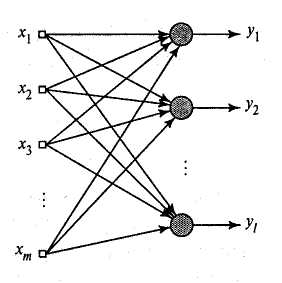
\includegraphics[height=6cm]{lec_neuro_14_8_6.png}
    \caption{Архитектура сети главных компонент}
    \label{lec_neuro_8_6}
\end{figure}

\begin{myquote}
    \textit{Lec\_Neuro\_14.docx}
\end{myquote}

Сеть главных компонент состоит из $m$ входных нейронов, обозначенных $x_i$.
Имеется единственный слой из $l$ нейронов $y_j$, каждый из которых обучается правилом Ойа. 
В синаптических весах каждого нейрона сохраняются направляющие косинусы соответствующего 
собственного вектора ковариационной матрицы. Матрица этих весов формирует базис размерностью $l<m$, 
повёрнутый относительно базиса входных признаков.

Размерность сигнального подпространства (пространства информативных признаков) определяется 
рангом ковариационной матрицы данных (\textit{в электронной версии это $l$}). МГК позволяет 
обнаружить наличие сильной корреляции в исходных признаках и, в силу этого, размерность
сигнального подпространства значительно меньше пространства входных признаков ($l \ll m$)
Каждый нейрон позволяет получить оценку дисперсии (собственные значения ковариационной 
матрицы данных) --- масштаба соответствующей оси.

В основе алгоритма обучения сети главных компонент лежит \textit{обобщенный алгоритм обучения Хебба} 
(Generalized Hebbian Algorithm, GHA).
Алгоритм устроен следующим образом:
\begin{equation}
    \Delta w _{ji}(n) = \eta 
    \left[
        y_j(n) x_i(n) - y_j(n) \sum_{k=1}^j w_{ki}(n) y_k(n) 
    \right], \quad i = 1, \dots, m,\quad j=1, \dots, l
    \label{eq:gha_seq}
\end{equation}

\noindent
где $\Delta w_{ji}(n)$ устанавливает связь между $x_i$ и $y_j$ и является \textit{величиной коррекции}
пред- и постсинаптических сигналов $x_i$ и $y_j$ соответственно.




\subsubsection{Последовательное обучение}

Для упрощения анализа на первом этапе примем предположим, что реализуется последовательное
во времени обучение (настройка параметров) линейных нейронов: сначала обучается 1-й линейный нейрон,
за ним 2-й линейный нейрон и т.д.

Рассмотрим обучение 1-го линейного нейрона. В этом случае $j=1$, а поскольку остальные нейроны
не используются, сумма в \ref{eq:gha_seq} вырождается в $\sum_{k=1}^1$ --- алгоритм вырождается 
в правило Ойа, реализующий 1-й и 2-й принципы самоорганизации (самоусиления [гипотеза корреляции, 
1-я компонента] и конкуренции).

Результатом является формирование в пространстве признаков оси, единичный орт которой указывает
направление первого главного собственного вектора ковариационной матрицы обучающего примера. 
При проекции этой оси на ось сигнального подпространства получим порцию полезной информации, 
которую даёт $j$-я ось сигнального подпространства.
Вдоль оси с $j=1$ степень рассеяния обучающих примеров наибольшая.

Далее из вектора обучающего примера $\vec{x}$ вычитаем фактическую реакцию, масштабированную вектором
синаптических весов --- проекцию его на ось сигнального подпространства:
\begin{equation}
    \vec{x}^\prime(n) = \vec{x}(n) - \vec{w}(n) y_1(n)
    \label{eq:first_main_comp}
\end{equation}

По сути, происходит "обеление" обучающего примера, из которого "удаляется" первая главная 
(информативная) компонента. Таким образом, второй нейрон ($j=2$) обрабатывает уже 
модифицированный вектор входных компонентов $\vec{x}'(n)$.
Разобьём сумму в \ref{eq:gha_seq} на 2 компоненты:

\begin{equation}
    \Delta w_{2i}(n) = \eta \cdot y_2(n) \left[
        x_i(n) - y_1(n) w_{1i}(n) - w_{2i}(n)
    \right]
\end{equation}

Введём новое обозначение:

\begin{equation}
    x_{2i}' = x_i(n) - w_{1i}(n) y_1(n)
    \label{eq:substit_oya}
\end{equation}

Тогда \ref{eq:gha_seq} для $j=2$ с учётом \ref{eq:substit_oya} становится аналогичным правилу Ойа:

\begin{equation}
    \Delta w_{2i}(n) = \eta \cdot y_2(n) 
    \left[
        x_{2i}'(n) - w_{2i}(n) y_2(n)
    \right]
\end{equation}

Удаление первой информативной компоненты \ref{eq:first_main_comp} приводит \ref{eq:gha_seq} 
к виду, аналогичному правилу обучения Ойа.

Повторив аналогично действия, удалим вторую главную компоненту из набора обучающих примеров 
для перехода к обучению 3-го нейрона, т.е. в гиперплоскости, образованной 1-м и 2-м собственным 
векторами, имея масштабированные вектора информативных признаков, их сумму удаляем из вектора 
обучающих примеров.

\begin{equation}
    \vec{x}^\prime(n) = \vec{x}(n) - \vec{w}(n) y_1(n) - \vec{w}(n) y_1(n) 
\end{equation}

Аналогичные действия повторяем и для третьего нейрона, что позволяет перейти к обучению 4-го
линейного нейрона. Т.е., в общем случае:

\begin{align}
    \Delta w_{ji}(n) = \eta \cdot y_j(n) 
    \left[
        x_{ji}'(n) - w_{ji}(n) y_j(n)
    \right], \quad i = 1, \dots, m,\quad j=1, \dots, l \\
    x_{ji}^\prime (n) = x_i(n) - \sum_{k=1}^{j-1} w_{ki} (n) y_k (n)
\end{align}

Итого получим, что в исходном пространстве сформирован базис сигнального подпространства
\begin{equation*}
    \vec{w}_1, \dots, \vec{w}_l,
\end{equation*}
\noindent
на который ортогонально спроецирован вектор обучающего примера, т.е. Реализована 
\textit{пространственная декомпозиция}.
Остаток (значение вектора обучающего примера после вычета всех главных компонент)
--- \textit{ошибка реконструкции данных}, --- вектор, который целиком содержится 
в шумовом подпространстве.

Анализ показывает, что такого рода процедура представляет собой декомпозицию исходных
признаков на информативные признаки в виде произведений собственных чисел ковариационной матрицы
(совпадают с $y_i$) на собственные вектора ковариационной матрицы $\vec{q}_i$.

Для получения оценки дисперсии ошибки реконструкции из каждого обучающего примера необходимо 
вычесть собственные вектора и просуммировать длины полученных векторов-остатков, либо
получить относительное значение, пользуясь значениями собственных чисел ковариационной матрицы:

\begin{equation}
    \dfrac{\sum_{k=l+1}^m \lambda_k}{\sum_{k=1}^m \lambda_k}
\end{equation}

\begin{figure}[htbp]
    \centering
    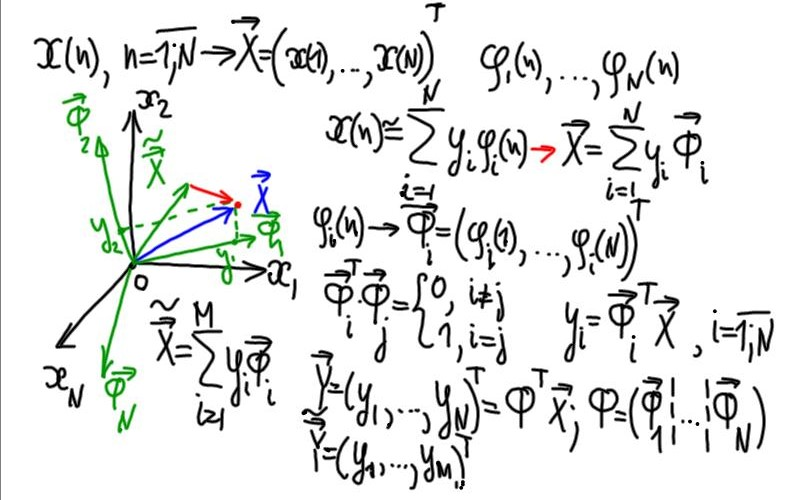
\includegraphics[height=6cm]{hyperflat_12_1.jpeg}
    \caption{hyperflat 12 1}
    \label{hyperflat_12_1}
\end{figure}




\subsubsection{Параллельное обучение}

Рассмотрим новые объекты анализа.

Сформируем матрицу единичных векторов синаптических весов сети главных компонент
размерности $l \times m$:
\begin{equation}
    \mathbf{W}(n) = 
    \left[
        \vec{w}_1(n), \vec{w}_2(n) , \dots, \vec{w}_l(n)
    \right]^T
\end{equation}

Заметим, что:
\begin{equation*}
    \mathbf{W}^T(n) = 
    \left\{
        w_{ji}(n)
    \right\}, \quad i = 1, \dots, m,\quad j=1, \dots, l
\end{equation*}

Вводится величина коррекции (\textit{обобщенный алгоритм Хебба в матричном виде}):
\begin{equation}
    (8.91)
    \Delta \mathbf{W}(n) = \mathbf{\eta}(n) 
    \left\{
        \vec{y}(n) \cdot \vec{x}^T(n) - LT
        \left[
            \vec{y}(n) \cdot \vec{y}^T(n)
        \right]
        \cdot \mathbf{W}(n)        
    \right\}
\end{equation}

\noindent
$\vec{y}(n)$ -- вектор-столбец с $l$ компонент, $\vec{x}(n)$ -- вектор-столбец с $m$ компонент,
$LT\left\{ \vec{y}(n) \cdot \vec{y}^T(n) \right\}$ --- оператор, устанавливающий все элементы 
матрицы $\vec{y}(n) \cdot \vec{y}^T(n)$, расположенные выше ее главной диагонали, в нуль
(формирует нижнюю треугольную матрицу).
Нижняя треугольная матрица необходима для реализации GHA. По мере обучения матрица и вектора 
обновляются.

\begin{myquote}
    \textit{Не уверен, но $\eta$ --- матрица}
\end{myquote}

Если параметр скорости обучения $\mathbf{\eta}(n)$ удовлетворяет условиям:
\begin{equation*}
    \lim_{n \to \infty} \mathbf{\eta}(n) = 0, \quad
    \sum_{n=0}^{\infty} \mathbf{\eta}(n) = \infty
\end{equation*}

\noindent
то обобщенный алгоритм Хебба будет сходиться к фиксированной точке, a $\mathbf{W}(n)$ сходится 
к матрице, строки которой являются первыми $l$ собственными векторами матрицы ковариации
размерности $m \times m$ входных векторов размерности $m \times 1$, упорядоченных по убыванию 
собственных значений.




\section{Лекция 28.05 (показаны новые наработки в 514м)}


\end{document}